\stepcounter{chapter}
\setcounter{eqtn}{0}

\raggedcolumns\setlength{\multicolsep}{-4mm}
\begin{multicols}{2}

\parbf{\ref{ex:ell-infty}.}
Проверьте все условия определения метрики на странице \pageref{page:def:metric}.

\parbf{\ref{ex:B2inB1}}; \ref{SHORT.ex:B2inB1:a}.
Заметьте, что $\dist{p}{q}{\spc{X}}\le 1$.
Применив неравенство треугольника, покажите, что $\dist{p}{x}{\spc{X}}\le 2$ для любого $x\in B[q,1]$.
Сделайте вывод. 

\parit{\ref{SHORT.ex:B2inB1:b}.}
Возьмите за $\spc{X}$ луч $[0,\infty)$ со стандартной метрикой; $p=0$ и $q=\tfrac45$.

\parbf{\ref{ex:shrt=>continuous}.}
Покажите, что условия в \ref{def:continuous} выполняются при $\delta=\epsilon$.

\parbf{\ref{ex:close-open}.}
Предположим, что дополнение $\Omega=\spc{X}\setminus Q$ открыто.
Тогда для каждой точки $p\in \Omega$ существует такое $\epsilon>0$, что $\dist{p}{q}{\spc{X}}>\epsilon$ для любого $q\in Q$.
Следовательно, $p$ \textit{не} может быть предельной точкой никакой последовательности из $Q$.
Значит, любой предел последовательности в $Q$ принадлежит $Q$,
и по определению, $Q$ замкнуто.

Теперь предположим, что $\Omega=\spc{X}\setminus Q$ не открыто.
Докажите, что существует точка $p\in \Omega$ и последовательность $q_n\in Q$ такая, что $\dist{p}{q_n}{\spc{X}}<\tfrac 1n$ для любого~$n$.
Выведите отсюда, что $q_n\to p$ при $n\to \infty$, и, значит, $Q$ незамкнуто.


%\end{multicols}
%\par\noindent\rule{\textwidth}{0.4pt}
%\begin{multicols}{2}

\stepcounter{chapter}
\setcounter{eqtn}{0}

\parbf{\ref{ex:9}}; \ref{SHORT.ex:9:compact}.
Воспользуйтесь тем, что непрерывное инъективное отображение, определённое на компактном множестве, является вложением (\ref{thm:Hausdorff-compact}).

\parit{\ref{SHORT.ex:9:9}.}
Образ $\gamma$ может выглядеть как цифры $8$ или $9$.

\parbf{\ref{ex:mono}.}
Сдавите окрестности концов в их концы.

\parbf{\ref{aex:simple-curve}.}
Пусть $\alpha$ --- путь, соединяющий $p$ с~$q$.
Можно предположить, что $\alpha(t)\ne p,q$ для $t\ne0,1$.

Назовём открытое множество $\Omega$ в $(0,1)$ {}\emph{подходящим},
если $\alpha(a)=\alpha(b)$ для любой компоненты связности $(a,b)$ в $\Omega$.
Покажите, что объединение, вложенных подходящих множеств, является подходящим.
Следовательно, найдётся максимальное подходящее множество $\hat \Omega$.

Определим $\beta(t)=\alpha(a)$ для любого $t$ в компоненте связности $(a,b)\subset\hat \Omega$, и $\beta (t) \z= \alpha (t) $ для $t\notin\hat{\Omega}$.
Заметьте, что для любого $x\in [0,1]$ множество $\beta^{-1}\{\beta(x)\}$ связно.


Остаётся получить простой путь, репараметризовав $\beta$.
Для этого нужно построить такую монотонную функцию $\tau\:[0,1]\z\to[0,1]$, что 
$\tau(t_1)\z=\tau(t_2)$ тогда и только тогда, когда существует компонента связности $(a,b)\subset\hat \Omega$ такая, что $t_1,t_2\z\in [a,b]$.

Функция $\tau$ похожа на так называемую {}\emph{чёртову лестницу};
разберитесь с её построением и воспользуйтесь им, чтобы построить $\tau$.

\parbf{\ref{ex:L-shape}.}
Обозначим объединение двух полуосей через~$L$.

Заметьте, что $f(t)\to\infty$ при $t\to \infty$.
Так как $f(0)=0$, по теореме о промежуточных значениях, $f(t)$ принимает все неотрицательные значения при $t\ge 0$.
Воспользуйтесь этим, чтобы показать, что $L$ есть образ~$\alpha$.

Далее, покажите, что функция $f$ строго возрастает при $t> 0$.
Выведите отсюда, что отображение $t\mapsto \alpha(t)$ инъективно.

Итак, $\alpha$ --- гладкая параметризация~$L$.

Теперь начнём с произвольной гладкой параметризации~$L$, скажем $\beta\:t\z\mapsto (x(t),y(t))$.
Можно считать, что $x(0)\z=y(0)=0$.
Заметим, что $x(t)\ge 0$ для любого $t$, следовательно, $x'(0)=0$.
Точно также получаем, что $y'(0)\z=0$.
То есть, $\beta'(0)=0$.
Значит, $L$ не допускает гладкой \textit{регулярной} параметризации.


\parbf{\ref{ex:cycloid}.}
Примените определения.
Для \ref{SHORT.ex:cycloid:regular} нужно проверить, что $\gamma'_\ell\ne 0$.
Для \ref{SHORT.ex:cycloid:simple} нужно проверить, что $\gamma_\ell(t_0)\z=\gamma(t_1)$ только если $t_0=t_1$.

\parbf{\ref{ex:nonregular}.}
Заметьте, что параметризация $t\mapsto (t,t^3)$ гладкая и регулярная.
Измените её так, чтобы скорость в одной из точек была равна нулю.

\begin{wrapfigure}{r}{20 mm}
\vskip-0mm
\centering
\includegraphics{mppics/pic-270}
\vskip-2mm
\end{wrapfigure}

\parbf{\ref{ex:y^2=x^3}.}
Это \index{полукубическая парабола}\emph{полукубическая парабола}; она показана на рисунке.
Попробуйте рассуждать аналогично \ref{ex:L-shape}.

\parbf{\ref{ex:viviani}.}
При $\ell=0$ система описывает пару точек $(0,0,\pm1)$, так что можно считать, что $\ell\z\ne 0$.

Первое уравнение описывает единичную сферу с центром в начале координат, а второе --- цилиндр над окружностью в плоскости $(x,y)$ с центром в точке $(-\tfrac\ell2,0)$ и радиусом~$|\tfrac\ell2|$.

Найдите градиенты $\nabla f$ и $\nabla h$ функций
\begin{align*}
 f(x,y,z)&=x^2+y^2+z^2-1,
 \\
 h(x,y,z)&=x^2+\ell\cdot x+y^2.
\end{align*}
Покажите, что при $\ell\ne 0$ градиенты линейно зависимы только на оси $x$.
Выведите отсюда, что для $\ell\ne\pm 1$ каждая компонента связности множества решений является гладкой кривой.

Покажите, что 
\begin{itemize}
\item если $|\ell|<1$, то множество имеет две связные компоненты с $z>0$ и $z<0$.
\item если же $|\ell|\ge1$, то множество связно.
\end{itemize}

Линейная независимость градиентов предоставляет лишь достаточное условие.
Поэтому случай $\ell=\pm1$ придётся проверить руками.
В этом случае окрестность точки $(\pm1,0,0)$ не допускает гладкой регулярной параметризации --- попробуйте это доказать.
Случай $\ell=1$ показан на рисунке.

\begin{Figure}
\centering
\vskip-0mm
\begin{lpic}[t(2mm),b(0mm),r(0mm),l(0mm)]{asy/viviani(1)}
\lbl[r]{-.5,18;$x$}
\lbl[l]{41,22;$y$}
\lbl[r]{18,54;$z$}
\end{lpic}
\end{Figure}

\parit{Замечание.}
При $\ell=\pm1$ получается так называемая \index{кривая Вивиани}\emph{кривая Вивиани}.
Она допускает следующую гладкую регулярную параметризацию с самопересечением в точке $(\pm1,0,0)$
\[t\mapsto(\pm(\cos t)^2,\cos t\cdot\sin t,\sin t).\]

\parbf{\ref{ex:open-curve}.}
Допустим, что $|\gamma(t)|\z\to\infty$ при $t\to\pm\infty$.
Выберем компактное множество $K\subset \mathbb{R}^3$.
Покажите, что прообраз $\gamma^{-1}(K)$ ограничен замкнут в $\mathbb{R}$,
и примените лемму Гейне --- Бореля (\ref{thm:Heine--Borel}).
Выведите, что $\gamma$ собственная.

Теперь предположим, что $\gamma(t_n)$ сходится для какой-то последовательности $t_n\to \pm \infty$; пусть $p$ --- её предел и $K$ --- замкнутый шар с центром в~$p$.
Убедитесь, что прообраз $\gamma^{-1}(K)$ некомпактен.
Выведите отсюда, что $\gamma$ несобственная.

\parbf{\ref{ex:proper-closed}.}
Докажите, что множество $C\subset \mathbb{R}^3$ является замкнутым тогда и только тогда, когда пересечение $K\cap C$ компактно для любого компактного $K\subset \mathbb{R}^3$,
и воспользуйтесь этим.

\parbf{\ref{ex:proper-curve}.}
Не умаляя общности, можно считать, что начало координат не лежит на кривой.

Покажите, что инверсия плоскости $(x,y)\z\mapsto (\tfrac{x}{x^2+y^2},\tfrac{y}{x^2+y^2})$ отображает нашу кривую в замкнутую кривую с удалённым началом координат.
Примените теорему Жордана для полученной кривой и снова воспользуйтесь инверсией.


%\end{multicols}
%\par\noindent\rule{\textwidth}{0.4pt}
%\begin{multicols}{2}

\stepcounter{chapter}
\setcounter{eqtn}{0}

\parbf{\ref{ex:integral-length-0}.}
Покажите, что если взять точную верхнюю грань в \ref{def:length} для всех последовательностей
$a=t_0\le t_1\le\z\dots\le t_k=b$, то результат будет тем же самым.

Предположим, что $\gamma_2$ --- репараметризация $\gamma_1$ с помощью $\tau\:[a_1,b_1]\to [a_2,b_2]$; не умаляя общности, можно считать, что $\tau$ неубывающая.
Пусть $\theta_i=\tau(t_i)$.
Заметьте, что $a_2=\theta_0\z\le\theta_1\le \z\dots\le\theta_k=b_2$ тогда и только тогда, когда 
$a_1=t_0\le t_1\le\z\dots\le t_k=b_1$.
Сделайте последний шаг.

\parbf{\ref{ex:length-chain}.}
Покажите, что для любой вписанной ломаной $\beta$ и любого $\epsilon>0$ выполняется
\[\length\beta_n>\length\beta-\epsilon.\]
при всех достаточно больших $n$.
Выведите отсюда, что
\[\liminf_{n\to\infty}\length\beta_n\ge \length \gamma.\]
Используя определение длины, покажите, что 
\[\limsup_{n\to\infty}\length\beta_n\le \length \gamma.\]
Убедитесь, что из полученных неравенств следует всё, что надо.

\parbf{\ref{ex:length-image}.}
Для данного разбиения $0=t_0<\z\dots <t_n\z=1$ отрезка $[0,1]$, положим $\tau_0=0$ и 
\[\tau_i=\max\set{\tau \in[0,1]}{\beta(\tau_i)=\gamma(t_i)}\]
при $i>0$.
Покажите, что $(\tau_i)$ является разбиением $[0,1]$;
то есть $0=\tau_0<\tau_1<\z\dots<\tau_n=1$.

По построению 
\begin{align*}
&|\gamma(t_0)-\gamma(t_1)|+|\gamma(t_1)-\gamma(t_2)|+\dots
\\
&\qquad\qquad\dots+|\gamma(t_{n-1})-\gamma(t_n)|=
\\
&=
|\beta(\tau_0)-\beta(\tau_1)|+|\beta(\tau_1)-\beta(\tau_2)|+\dots
\\
&\qquad\qquad\dots+|\beta(\tau_{n-1})-\beta(\tau_n)|.
\end{align*}
Поскольку разбиение $(t_i)$ произвольно, получаем 
\[\length \beta\ge \length \gamma.\]

\parit{Замечания.}
Полезно сравнить это упражнение с \ref{obs:S2-length}.

Неравенство может оказаться строгим.
Такое происходит, если $\beta$ ходит вдоль $\gamma$ туда-сюда.
В этом случае разбиение $(\tau_i)$ выше нельзя выбрать произвольно.

В предположении $\beta([0,1])\z\supset\gamma([0,1])$, задача решается применением следующего неравенства \cite[2.6.1+2.6.2]{burago-burago-ivanov}:
\[h\le \length\gamma,\] где $h$ --- одномерная мера Хаусдорфа образа $\gamma([0,1])$.
Более того, равенство достигается тога и только тогда, когда $\gamma$ простая.

\parbf{\ref{ex:integral-length}}; \ref{SHORT.ex:integral-length>}.
Примените основную теорему анализа к каждому отрезку разбиения.

\parit{\ref{SHORT.ex:integral-length<}.}
Рассмотрите разбиение, для которого вектор скорости $\alpha'(t)$ почти постоянен на каждом из отрезков.

\parbf{\ref{adex:integral-length}.}
Воспользуйтесь теоремами Радемахера и Лузина (\ref{thm:rademacher} и \ref{thm:lusin}).

\parbf{\ref{ex:nonrectifiable-curve}}; \ref{SHORT.ex:nonrectifiable-curve:a}.
Посмотрите на рисунок и догадайтесь как запараметризовать дугу снежинки отрезком $[0,1]$.
Расширьте параметризацию на всю снежинку.
Убедитесь, что она действительно описывает вложение окружности в плоскость.

\begin{Figure}
\vskip-0mm
\centering
\includegraphics{mppics/pic-226}
\vskip0mm
\end{Figure}

\parit{\ref{SHORT.ex:nonrectifiable-curve:b}.}
Пусть $\gamma\:[0,1]\to\mathbb{R}^2$ --- спрямляемая кривая, и $\gamma_k$ --- её гомотетия с коэффициентом $k>0$;
то есть $\gamma_k(t)=k\cdot\gamma(t)$ для любого~$t$.
Покажите, что 
\[\length\gamma_k=k\cdot\length \gamma.\]

Теперь допустим, что дуга $\gamma$ снежинки Коха, показанная на рисунке, спрямляема,
и $\ell$ --- её длина.
Заметьте, что $\gamma$ можно разделить на 4 дуги, каждая из которых конгруэнтна гомотетии $\gamma$ с коэффициентом~$\tfrac13$.
Следовательно, $\ell=\tfrac43\cdot\ell$,
но ведь $\ell>0$ --- противоречие.

\parbf{\ref{ex:cont-length}.}
Применив \ref{thm:length-semicont}, покажите, что $s$ полунепрерывна снизу;
то есть если $t_n\to t_\infty$ при $n\to\infty$, тогда 
\[\liminf_{n\to\infty} s(t_n)\ge s(t_\infty).\]
Убедитесь, что
\[s(t)=s(b)-\length(\gamma|_{[t,b]}).\]
Применив это равенство с \ref{thm:length-semicont}, покажите, что $s$ полунепрерывна сверху.
Выведите отсюда, что функция $s$ непрерывна.
Наконец, покажите, что $s$ неубывающая, 
и воспользуйтесь этим.

\parbf{\ref{ex:arc-length-helix}.} 
Можно предположить, что $a\ne 0$ или $b\ne 0$,
иначе задача тривиальна.

Покажите, что $|\gamma'(t)|\equiv \sqrt{a^2+b^2}$;
в частности, скорость постоянна.
Значит, $s\z=t/\sqrt{a^2+b^2}$ --- параметр длины.
Остаётся подставить $s\cdot \sqrt{a^2+b^2}$ вместо~$t$.


\parbf{\ref{ex:convex-hull}.}
Пусть $p_1\dots p_n$ --- замкнутая ломаная, вписанная в $\beta$.
По \ref{cor:convex=>rectifiable}, можно считать, что её длина сколь угодно близка к длине $\beta$;
то есть
\[\length (p_1\dots p_n)>\length\beta-\epsilon\]
для любого наперёд заданного $\epsilon>0$.

Убедитесь, что при всём при этом можно предположить, что каждая точка $p_i$ лежит на $\alpha$.

Поскольку $\alpha$ простая, точки $p_1,\dots,p_n$ появляются на $\alpha$ в одном и том же циклическом порядке;
то есть ломаная $p_1\dots p_n$ также вписана в $\alpha$.
В частности,
\[\length\alpha\ge \length (p_1\dots p_n).\]
Следовательно, 
\[\length\alpha>\length\beta-\epsilon.\]
для любого $\epsilon>0$.
Отсюда
\[\length\alpha\ge\length\beta.\]

\begin{wrapfigure}{r}{25 mm}
\vskip-0mm
\centering
\includegraphics{mppics/pic-275}
\vskip0mm
\end{wrapfigure}

Если у $\alpha$ есть самопересечения, то точки $p_1,\dots, p_n$ могут располагаться на $\alpha$ в другом циклическом порядке, скажем, $p_{i_1},\dots,p_{i_n}$.
Примените неравенство треугольника, чтобы показать, что
\[\length(p_{i_1}\dots p_{i_n})\ge \length (p_1\dots p_n)\]
и воспользуйтесь этим, чтобы обобщить доказательство.

\parbf{\ref{ex:convex-croftons}.} 
Обозначим через $\ell_{\vec u}$ отрезок, 
полученный ортогональной проекцией $\gamma$ на прямую в направлении ${\vec u}$.
Поскольку $\gamma_{\vec u}$ проходит вдоль $\ell_{\vec u}$ туда и обратно, получаем
\[\length\gamma_{\vec u}\ge 2\cdot\length\ell_{\vec u}.\]
По формуле Крофтона, 
\[\length\gamma\ge \pi\cdot \overline{\length\ell_{\vec u}}.\]

В случае равенства кривая $\gamma_{\vec u}$ проходит точно туда и обратно вдоль $\ell_{\vec u}$ без дополнительных зигзагов;
это должно происходить для почти всех (а следовательно, и для всех) направлений~${\vec u}$.

Пусть $K$ --- замкнутое множество, ограниченное~$\gamma$.
Последнее утверждение означает, что если прямая пересекает $K$, то пересечение отрезок или точка.
Отсюда следует, что $K$ выпукло.

\parbf{\ref{adex:more-croftons}.}
Доказательство то же, что у обычной формулы Крофтона.
Чтобы найти коэффициенты, достаточно проверить её на единичном интервале,
и это делается интегрированием
\begin{align*}
\frac1{k_1}&=\frac{1}{\area \mathbb{S}^2}\cdot\iint_{\mathbb{S}^2} |x|;
\\
\frac1{k_2}&=\frac{1}{\area \mathbb{S}^2}\cdot\iint_{\mathbb{S}^2} \sqrt{1-x^2}.
\end{align*}
Ответы: $k_1=2$ и $k_2=\tfrac4\pi$.

\parbf{\ref{ex:intrinsic-convex}.}
Необходимость очевидна.
Чтобы доказать достаточность, допустим, что $A$ не выпукло;
то есть найдутся точки $x,y\in A$ и точка $z\notin A$, которая лежит между $x$ и~$y$.

Так как $A$ замкнуто, его дополнение открыто.
Иными словами, существует шар $B(z,\epsilon)$, который не пересекает $A$ для некоторого $\epsilon>0$.

Покажите, что найдётся такое $\delta>0$, что любая кривая из $x$ в $y$ длины не более $\dist{x}{y}{\mathbb{R}^3}+\delta$ задевает $B(z,\epsilon)$.
Отсюда $\dist{x}{y}A\z\ge \dist{x}{y}{\mathbb{R}^3}+\delta$; 
в частности, $\dist{x}{y}A\ne \dist{x}{y}{\mathbb{R}^3}$.

\begin{wrapfigure}{r}{23 mm}
\vskip-4mm
\centering
\includegraphics{mppics/pic-280}
\vskip0mm
\end{wrapfigure}

\parbf{\ref{ex:antipodal}.}
Сферическая кривая, показанная на рисунке, не имеет антиподальных пар точек.
Однако на одной из её сторон лежат три точки $x,y,z$ с одного экватора, а на другой --- их антиподы $-x,-y,-z$.
(Мы предполагаем, что точки $x,-y,z,-x,y,-z$ лежат в этом же порядке на экваторе.)

Покажите, что такая кривая не может лежать ни в одной полусфере.

\parbf{\ref{ex:bisection-of-S2}.}
Допустим, что $\gamma$ лежит в открытой полусфере (\ref{lem:hemisphere}).
В частности, она не делит $\mathbb{S}^2$ на две области равной площади --- противоречие.

\parbf{\ref{ex:flaw}.}
Уже первое предложение неверно --- \textit{недостаточно} показать, что диаметр не превышает~2.
Например, если у равностороннего треугольника радиус описанной окружности чуть больше 1,
то его диаметр (который определяется как максимальное расстояние между его точками) будет чуть больше $\sqrt3$, так что он меньше 2.

С другой стороны, доказательство леммы о полусфере (\ref{lem:hemisphere}) можно приспособить для получения правильного решения.
А именно: (1) выберите две точки $p$ и $q$ на $\gamma$, которые делят её на две дуги одинаковой длины;
(2) пусть $z$ --- средина между $p$ и $q$;
(3) покажите, что $\gamma$ лежит в единичном круге с центром в~$z$.

\parbf{\ref{adex:crofton}}; \ref{SHORT.adex:crofton:crofton}.
Рассуждение схоже с доказательством обычной формулы Крофтона (\ref{sec:crofton}).

\parit{\ref{SHORT.adex:crofton:hemisphere}.}
Предположим, что $\length \gamma<2\cdot\pi$.
Согласно \ref{SHORT.adex:crofton:crofton},
\[\overline{\length \gamma^*_{\vec u}}<2\cdot\pi.\]
Следовательно, 
\[\length \gamma^*_{\vec u}<2\cdot\pi\]
для некоторого ${\vec u}$. 

Заметьте, что $\gamma^*_{\vec u}$ идёт по некоторой полуокружности~$h$.
Следовательно, $\gamma$ лежит в полусфере, построенной на $h$ как на диаметре.

%\end{multicols}
%\par\noindent\rule{\textwidth}{0.4pt}
%\begin{multicols}{2}

\stepcounter{chapter}
\setcounter{eqtn}{0}

\parbf{\ref{ex:zero-curvature-curve}.}
Пусть кривая $\gamma$ имеет единичную скорость и нулевую кривизну. 
Тогда $\gamma''\equiv 0$, и, значит, вектор скорости $\vec v=\gamma'$ не меняется.
Отсюда, $\gamma(t)\z=p+(t-t_0)\cdot \vec v$, где $p=\gamma(t_0)$.

\parbf{\ref{ex:scaled-curvature}.} 
Заметьте, что $\alpha(t)\df\gamma_{\lambda}(t/\lambda)$ --- это параметризация кривой $ \gamma_{\lambda}$ с единичной скоростью,
и примените дважды правило дифференцирования сложной функции.

\parbf{\ref{ex:curvature-of-spherical-curve}.}
Продифференцируйте тождество $\langle\gamma(s),\gamma(s)\rangle=1$ несколько раз.

\parbf{\ref{ex:curvature-formulas}.} 
Пусть $\tan=\tfrac{\gamma'}{|\gamma|}$.
Выведите  тождества
\begin{align*}
\gamma''-(\gamma'')^\perp&=\tan\cdot\langle\gamma'',\tan\rangle,
&
|\gamma'|&=\sqrt{\langle \gamma',\gamma'\rangle},
\end{align*}
и воспользуйтесь ими.

\parbf{\ref{ex:curvature-graph}.} 
Примените \ref{ex:curvature-formulas:a} к параметризации $t\z\mapsto (t,f(t))$.

\parbf{\ref{ex:approximation-const-curvature}.}
Не умаляя общности, можно предположить, что у $\gamma$ единичная скорость.

Заметьте, что касательная индикатриса $\tan(s)\z=\gamma'(s)$ --- сферическая кривая и $|\tan'|\le 1$.
Воспользуйтесь этим для построения последовательности сферических кривых с единичной скоростью $\tan_n\:\mathbb{I}\to\mathbb{S}^2$ таких, что $\tan_n(s)\to \tan(s)$ при $n\to\infty$ для любого~$s$.
Покажите, что следующая последовательность кривых даёт решение
\[\gamma_n(s)=\gamma(a)+\int_a^s\tan_n(t)\cdot dt.\]

\parbf{\ref{ex:no-parallel-tangents}.}
Воспользуйтесь построением в \ref{ex:antipodal}, дабы получить замкнутую гладкую простую сферическую кривую $\tan\:\mathbb{S}^1\z\to\mathbb{S}^2$, которая не содержит пар антиподальных точек и имеет нулевое среднее значение.
Затем постройте кривую с касательной индикатрисой $\tan$.

\parit{Источник:}
Эту кривую построил Беньям\'{и}но С\'{е}гре \cite{segre}.

\parbf{\ref{ex:helix-curvature}.}
Покажите, что $\gamma_{a,b}''\perp \gamma'_{a,b}$, и примените \ref{ex:curvature-formulas:a}.

\parbf{\ref{ex:length>=2pi}.}
Примените теорему Фенхеля.

\parbf{\ref{ex:gamma/|gamma|}.}
Можно предположить, что у $\gamma$ единичная скорость.
Тогда $\langle\tan,\tan\rangle=1$ и  $\tan'\perp \tan$.
Пусть $\theta(s)=\measuredangle(\gamma(s),\gamma'(s))$ и, значит, $\langle \tan,\sigma\rangle=\cos\theta$.
Поэтому
\begin{align*}
\kur\cdot \sin\theta
&=|\tan'|\cdot \sin\theta\ge
-\langle \tan',\sigma\rangle=
\\
&=
\langle \tan,\sigma'\rangle-\langle \tan,\sigma\rangle'=
\\
&=
(|\sigma'|+\theta')\cdot \sin\theta.
\end{align*}
Следовательно, $\kur\ge |\sigma'|+\theta'$,
если $\theta\ne0,\pi$.
Остаётся проинтегрировать это неравенство и показать, что множество, для которого $\theta\z\ne0$ или $\pi$, не создаёт проблем.

\parit{Другое решение} строится на основе \ref{prop:inscribed-total-curvature}.

\parbf{\ref{ex:DNA}}; \ref{SHORT.ex:DNA:c''c>=k}.
Поскольку $|\gamma(s)|\le 1$, 
\begin{align*}
\langle\gamma''(s),\gamma(s)\rangle&\ge -|\gamma''(s)|\cdot|\gamma(s)|\ge-\kur(s)
\end{align*}
при всех~$s$.

\parit{\ref{SHORT.ex:DNA:int>=length-tc}.}
Поскольку $\gamma$ параметризована длиной, $\ell\z=\length\gamma$ и $\langle\gamma',\gamma'\rangle\equiv1$.
Следовательно,
\begin{align*}
\int_0^\ell\langle\gamma(s),\gamma'(s)\rangle'\cdot ds&=\\
=\int_0^\ell\langle\gamma'(s),\gamma'(s)\rangle\cdot ds&+\int_0^\ell\langle\gamma(s),\gamma''(s)\rangle\cdot ds\ge
\\
&\ge \length\gamma-\tc\gamma.
\end{align*}

\parit{\ref{SHORT.ex:DNA:end}.}
По основной теореме анализа,
\begin{align*}
\int_0^\ell\langle\gamma(s),\gamma'(s)\rangle'\cdot ds
&=\langle\gamma(s),\gamma'(s)\rangle\bigg|_0^\ell.
\end{align*}
Поскольку $\gamma(0)=\gamma(\ell)$ и $\gamma'(0)=\gamma'(\ell)$, правая часть равенства обращается в ноль.

Можно считать, что кривая в \ref{thm:DNA} описывается петлёй $\gamma\:[0,\ell]\to\mathbb{R}^3$, параметризованной длиной и ещё, что центр шара находится в начале координат, то есть $|\gamma|\le 1$.
Поскольку $\gamma$ гладкая и замкнутая, 
$\gamma'(0)=\gamma'(\ell)$ и $\gamma(0)=\gamma(\ell)$.
Следовательно, \ref{SHORT.ex:DNA:int>=length-tc} и \ref{SHORT.ex:DNA:end} влекут \ref{thm:DNA}.

\parbf{\ref{ex:tangent-support}.}
Покажите, что никакая прямая, отличная от $\ell$, не может подпирать $F$ в точке~$p$. 
Примените \ref{lem:separation}, чтобы показать, что какая-то прямая подпирает $F$ в точке $p$.
Сделайте вывод.

{

\begin{wrapfigure}{r}{22 mm}
\vskip-6mm
\centering
\includegraphics{mppics/pic-255}
\vskip0mm
\end{wrapfigure}

\parbf{\ref{ex:anti-bow}.}
Начнём с кривой $\gamma_1$, изображённой на рисунке.
Чтобы получить $\gamma_2$, слегка распрямите пунктирную дугу (то есть уменьшите её кривизну).

}

\parbf{\ref{ex:bow'}}; \ref{SHORT.ex:bow'+}.
Не умаляя общности, можно предположить, что $p=\gamma_1(a)\z=\gamma_2(a)$ --- начало координат, 
вектор $\vec u=\tan_1(a)\z=\tan_2(a)$ направлен вдоль оси $x$,
а точки $q_1=\gamma_1(b)$ и $q_2=\gamma_2(b)$ лежат в верхней полуплоскости $(x,y)$.

Допустим, что $\alpha_1<\alpha_2$.
Найдите такую точку $x$, что
$\dist{x}{q_1}{}<\dist{x}{q_2}{}$, и
$\gamma_1$ вместе с отрезками $[p,x]$ и $[x,q_1]$ ограничивает выпуклую область в $(x,y)$-плоскости.
(Здесь понадобится, что $\beta_1\le\tfrac\pi2$.)

Проверьте, что доказательство леммы о луке (\ref{lem:bow}) работает для произведений $[x,p]$ с $\gamma_1$ и $\gamma_2$, и придите к противоречию.

\parit{\ref{SHORT.ex:bow'-}.}
Посмотрите на рисунок и подумайте.

\begin{Figure}
\vskip-0mm
\centering
\includegraphics{mppics/pic-257}
\vskip0mm
\end{Figure}

\parit{Замечание.}
Это упражнение полезно сравнить с леммой о хорде (\ref{lem:chord}).

\parbf{\ref{ex:length-dist}}; \ref{SHORT.ex:length-dist:>}.
Выберите значение $s_0\in[a,b]$, которое делит полную кривизну $\gamma$ пополам.
Заметьте, что $\measuredangle(\gamma'(s_0),\gamma'(s))\le \theta$ для любого~$s$.
Используйте это неравенство так же, как в доказательстве леммы о луке.

\begin{wrapfigure}[3]{r}{22 mm}
\vskip-5mm
\centering
\includegraphics{mppics/pic-290}
\vskip-0mm
\end{wrapfigure}

\parit{\ref{SHORT.ex:length-dist:self-intersection:>pi}.}
Воспользуйтесь \ref{SHORT.ex:length-dist:>} и посмотрите на рисунок.


\parit{\ref{SHORT.ex:length-dist:=}.}
Начните с ломаной из двух звеньев равной длины и с внешним углом $2\cdot\theta$ и сгладьте вершину, используя срезки и сглаживания (\ref{sec:analysis}).

\parbf{\ref{ex:schwartz}.}
Пусть $\ell=\length\gamma$.
Допустим, что $\ell_1\z<\ell<\ell_2$, и пусть $\gamma_1$ --- дуга единичной окружности длины $\ell$.

Покажите, что расстояние между концами $\gamma_1$ больше, чем $|p-q|$, и примените лемму о луке (\ref{lem:bow}).

\parit{Источник:} Это утверждение приписывается Герману Шварцу \cite{shur}.

\parbf{\ref{ex:loop}.}
Допустим, что $\length\gamma<2\cdot\pi$. 
Примените лемму о луке (\ref{lem:bow}) к $\gamma$ и дуге единичной окружности той же длины.

\parbf{\ref{ex:bow-upper}.}
Выберите гладкую сферическую кривую $\alpha$, которая всё время идёт близко к одной точке;
например, маленькую сферическую окружность с центром в этой точке.
Рассмотрите кривую $\tan$, которая идёт по $\alpha$ со скоростью $\kappa(s)$ при любом $s\in [0,\ell]$.
Покажите, что кривая с касательной индикастрой $\tan$ решает задачу.

\parbf{\ref{ex:gromov-twist}.}
Можно предположить, что $\gamma$ имеет единичную скорость.
Допустим, что неравенство не выполняется при $t=0$.
Можно предположить, что $\alpha(0)\le\tfrac\pi2$;
в противном случае развернём параметризацию.

В плоскости, натянутой на вектора $\gamma(0)$ и $\gamma'(0)$, выберите дугу окружности (или отрезок прямой) $\sigma$ с единичной скоростью от $0$ до $\gamma(0)$, которая приходит в $\gamma(0)$ в направлении, противоположном $\gamma'(0)$.
Рассмотрите полуокружность $\tilde\gamma$ с единичной скоростью и кривизной $2$, которая начинается в $\gamma(0)$ в направлении $\gamma'(0)$ так, что произведение $\sigma*\tilde\gamma$ является дугой выпуклой плоской кривой; см. рисунок.

\begin{Figure}
\vskip-1mm
\centering
\includegraphics{mppics/pic-282}
\vskip-1mm
\end{Figure}

Покажите, что если $|\gamma(0)|> \sin[\alpha(0)]$, то $\tilde\gamma$ выходит за пределы единичного шара; то есть $|\tilde\gamma(t_0)|>1$ для некоторого $t_0$.

Произведения $\sigma*\gamma$ и $\sigma*\tilde\gamma$ не являются гладкими на стыке, но они дифференцируемы в этой точке.
Проверьте, что доказательство леммы о луке работает и в этом более общем случае.

Применив этот вариант леммы о луке к $\sigma*\gamma$ и $\sigma*\tilde\gamma$, получите, что $|\gamma(t_0)|\ge |\tilde\gamma(t_0)|$, и придите к противоречию.

\parit{Источник:} Это утверждение использовалось первым автором \cite{petrunin2023}.


%\end{multicols}
%\par\noindent\rule{\textwidth}{0.4pt}
%\begin{multicols}{2}

\stepcounter{chapter}
\setcounter{eqtn}{0}

\parbf{\ref{ex:chord-lemma-optimal}.} 
Пусть $\alpha=\measuredangle(\vec u,\vec w)$ 
и $\beta=\measuredangle(\vec w,\vec v)$.
Попробуйте догадаться до примера по рисунку.

\begin{Figure}
\vskip-1mm
\centering
\includegraphics{mppics/pic-285}
\vskip-1mm
\end{Figure}

Показанная кривая разделена на три дуги: I, II и III. 
Дуга I поворачивает от $\vec u$ к $\vec w$;
её полная кривизна равна $\alpha$.
Аналогично, дуга III поворачивает от $\vec w$ к $\vec v$ и имеет полную кривизну $\beta$. 
Дуга II проходит очень близко и почти параллельно хорде $pq$, и её полную кривизну можно сделать произвольно малой.

\parbf{\ref{ex:monotonic-tc}.}
Используйте, что внешний угол треугольника равен сумме внутренних углов в двух других вершинах.
Во второй части примените индукцию по числу вершин.

\parbf{\ref{ex:sef-intersection}.}
Допустим, что $x$ --- это точка самопересечения.
Покажите, что можно выбрать такие две точки $y$ и $z$ на $\gamma$ между самопересечениями, чтобы треугольник $xyz$ оказался невырожденным.
В частности, 
$\measuredangle\hinge yxz
\z+
\measuredangle\hinge zyx
<\pi$, или, что эквивалентно, $\tc{xyzx}\z>\pi$ для \textit{незамкнутой} вписанной ломаной $xyzx$.
Остаётся применить~\ref{prop:inscribed-total-curvature}.

\parbf{\ref{ex:quadrisecant}.}
Рассмотрим замкнутую ломаную $acbd$.
Убедитесь, что $\tc{acbd}\z=4\cdot\pi$, и примените \ref{prop:inscribed-total-curvature}.

\parit{Замечания.}
Прямые, пересекающие кривую, как в этом упражнении, называются \index{четырёхкратная секущая}\emph{альтернированными четырёхкратными секущими}.
Известно, что такая секущая найдётся у любого {}\emph{нетривиального узла} \cite{denne};
согласно упражнению, это доказывает так называемую {}\emph{теорему Фари --- Милнора} --- \textit{полная кривизна любого узла больше, чем~$4\cdot \pi$}; см. \cite{petrunin-stadler} и тамошние ссылки.

\parbf{\ref{ex:total-curvature=}.}
Согласно \ref{prop:inscribed-total-curvature}, $\tc\gamma\ge \tc\beta$;
остаётся показать, что
$\tc\gamma\le\sup\{\tc\beta\}$.
Другими словами, 
для любого $\epsilon>0$ и ломаной $\sigma=\vec u_0\dots \vec u_k$, вписанной в касательную индикатрису $\tan$ кривой $\gamma$, 
нам нужно построить такую ломаную $\beta$, вписанную в $\gamma$, что
\[\length\sigma<\tc\beta+\epsilon.
\eqlbl{eq:tc=<tc}\]

Предположим, что $\vec u_i=\tan(s_i)$.
Выберите вписанную ломаную $\beta=p_0\dots p_{2\cdot k+1}$ так, чтобы точки $p_{2\cdot i}$ и $p_{2\cdot i+1}$ лежали достаточно близко к $\gamma(s_i)$; этим можно добиться того, что направление вектора $p_{2\cdot i+1}-p_{2\cdot i}$ достаточно близко к вектору $\vec u_i$ для каждого~$i$.
Покажите, что \ref{eq:tc=<tc} выполняется для построенной ломаной~$\beta$.

\parbf{\ref{ex:tc-rectifiable}.}
Покажите, что для любой ломаной $\beta$, лежащей в шаре радиуса $R$, выполняется неравенство
\[\tc{\beta}+2\cdot \pi\ge\frac{\length\beta}R.\]
Убедитесь, что $\gamma$ лежит в каком-то шаре, и примените это неравенство.

Пример для второй части можно найти среди логарифмических спиралей.


%\end{multicols}
%\par\noindent\rule{\textwidth}{0.4pt}
%\begin{multicols}{2}

\stepcounter{chapter}
\setcounter{eqtn}{0}

\parbf{\ref{ex:helix-torsion}.} 
Параметр длины $s$ уже найден в \ref{ex:arc-length-helix}.
Остаётся вычислить базис Френе, кривизну и кручение.

{

\begin{wrapfigure}{r}{25 mm}
\vskip-3mm
\centering
\begin{lpic}[t(-0mm),b(0mm),r(0mm),l(0mm)]{asy/helix(1)}
\lbl[br]{8,24;$\norm$}
\lbl[b]{2,26;$\bi$}
\lbl[wl]{15,25;$\tan$}
\end{lpic}
\vskip-0mm
\end{wrapfigure}

Должно получится
\begin{align*}
\tan(t)&=\tfrac{(-a\cdot\sin t, a\cdot\cos t,b)}{\sqrt{a^2+b^2}},
\\
\norm(t)&=(-\cos t,-\sin t,0),
\\
\bi(t)&=\tfrac{(b\cdot \sin t,-b\cdot \cos t, a)}{\sqrt{a^2+b^2}},
\\
\kur(t) &\equiv \tfrac{a}{a^2+b^2},
\\
\tor(t) &\equiv \tfrac{b}{a^2+b^2}.
\end{align*}

Остаётся показать, что отображение $(a,b) \z\mapsto (\frac{a}{a^2+b^2}, \frac{b}{a^2+b^2})$ биективно отображает полуплоскость $a>0$ на себя.

}

\parbf{\ref{ex:beta-from-tau+nu}.}
По правилу произведения получаем
\begin{align*}
\bi'&=(\tan\times \norm)'=
\tan'\times \norm+\tan\times\norm'.
\end{align*}
Остаётся подставить значения из \ref{eq:frenet-tau} и \ref{eq:frenet-nu} и упростить.

\parbf{\ref{ex:torsion=0}.}
Воспользуйтесь уравнением $\bi' = - \tor\cdot \norm $.

\parbf{\ref{ex:+B}.}
Можно считать, что $\gamma_0$ параметризована длиной.
Покажите, что
$|\gamma_1'|=|\tan-\tor\cdot \norm|\ge 1$ и используйте это.

\parbf{\ref{ex:frenet}.}
$\tfrac{\gamma'\times\gamma''}{|\gamma'\times\gamma''|}$ --- единичный вектор, перпендикулярный плоскости, натянутой на $\gamma'$ и $\gamma''$.
Поэтому, с точностью до знака, он равен $\bi$.
Остаётся найти знак.

\parbf{\ref{ex:moment-curve}.}
Примените \ref{ex:curvature-formulas:b} и \ref{ex:frenet}.

\parbf{\ref{ex:bow-converse}.}
Можно считать, что $t_0=0$ и $\gamma_i(0)\z=0$.
Рассмотрим функции
\begin{align*}
\rho_i(t)&\df|\gamma_i(t)|^2=\langle \gamma_i(t),\gamma_i(t)\rangle.
\end{align*}
Заметьте, что $\rho_1\ge \rho_2$ и $\rho_i(0)=0$.
Убедитесь, что 
\begin{align*}
\rho_i'(0)&=0,
&
\rho_i''(0)&=2,
\\
\rho_i'''(0)&=0,
&
\rho_i''''(0)&=-2\cdot\kur(0)^2_{\gamma_i}.
\end{align*}
Сделайте вывод. (Сравните с \ref{ex:const-dist}.)

\parbf{\ref{ex:torsion-indicatrix}.}
Допустим, что касательная индикатриса не имеет самопересечений.
Покажите, что она лежит в открытой полусфере, и рассуждайте, как в теореме Фенхеля.

\parbf{\ref{ex:lancret}}; \ref{SHORT.ex:lancret:a}.
Заметьте, что 
$\langle \vec w,\tan\rangle'=0$.
Выведите отсюда, что $\langle \vec w, \norm\rangle =0$.
Далее, покажите, что $\langle \vec w, \tan\rangle^2+\langle \vec w, \bi\rangle^2=\langle \vec w, \vec w\rangle$, и воспользуйтесь этим.
При доказательстве последнего тождества примените формулу Френе для~$\norm'$.

\parit{\ref{SHORT.ex:lancret:b}.}
Покажите, что $\vec w'=0$;
это означает, что $\langle \vec w,\tan\rangle\z=\tfrac\tor\kur$.
В частности, вектор скорости образует постоянный угол с $\vec w$; то есть $\gamma$ --- линия откоса.

\parbf{\ref{ex:evolvent-constant-slope}.}
Пусть $\alpha$ --- эвольвента кривой $\gamma$, а $\vec w$ --- фиксированный вектор.
Покажите, что скалярное произведение $\langle \vec w,\alpha\rangle$ постоянно, если $\gamma$ идёт под постоянным углом к $\vec w$, и воспользуйтесь этим.

\parbf{\ref{ex:spherical-frenet}}.
Часть \ref{SHORT.ex:spherical-frenet:tau} следует из того, что $(\tan,\norm,\bi)$ является ортонормированным базисом.
Для \ref{SHORT.ex:spherical-frenet:nu} возьмите первую и вторую производные от тождества $\langle\gamma,\gamma\rangle=1$ и упростите их, пользуясь формулами Френе.
Часть \ref{SHORT.ex:spherical-frenet:beta} вытекает из \ref{SHORT.ex:spherical-frenet:nu} и формул Френе.
Согласно \ref{SHORT.ex:spherical-frenet:beta}, $\int\tfrac\tor\kur=0$, следовательно, выполняется \ref{SHORT.ex:spherical-frenet:beta+}.
Часть \ref{SHORT.ex:spherical-frenet:kur-tor} доказывается алгебраическими манипуляциями.
В \ref{SHORT.ex:spherical-frenet:f},
воспользовавшись формулами Френе, покажите, что $(\gamma+\tfrac1\kur\cdot \norm+\tfrac{\kur'}{\kur^2\cdot\tor}\cdot\bi)'=0$.

\parit{Замечание.}
Из \ref{SHORT.ex:spherical-frenet:beta} получаем, что \textit{$\int\tfrac\tor\kur=0$ для любой замкнутой гладкой сферической кривой}.
Известно, что это свойство характеризует сферы и плоскости; это доказано Беньямино Сегре \cite{segre}.

\parbf{\ref{ex:cur+tor=helix}.}
Воспользуйтесь второй частью \ref{ex:helix-torsion}.

\parbf{\ref{ex:const-dist}.}
По условию,
\begin{align*}
\rho(\ell)&=|\gamma(t+\ell)-\gamma(t)|^2=
\\
&=\langle \gamma(t+\ell)-\gamma(t),\gamma(t+\ell)-\gamma(t)\rangle
\end{align*}
--- гладкая функция, не зависящая от~$t$.
Выразите скорость, кривизну и кручение $\gamma$ через производные $\rho^{(n)}(0)$.
Будьте терпеливы, потребуются две производные для скорости,
четыре для кривизны,
и шесть для кручения.
После этого, примените \ref{ex:cur+tor=helix}.


%\end{multicols}
%\par\noindent\rule{\textwidth}{0.4pt}
%\begin{multicols}{2}

\stepcounter{chapter}
\setcounter{eqtn}{0}

\parbf{\ref{ex:bike}.}
Можно считать, что $\gamma_0$ параметризована длиной.
Тогда
\begin{align*}
|\gamma_1'|&=|\gamma_0'+\tan'|=|\tan+\kur\cdot\norm|.
\end{align*}
Отсюда 
\[|\gamma_1'(t)|\ge|\gamma_0'(t)|
\quad\text{и}\quad
|\gamma_1'(t)|\ge|\kur(t)_{\gamma_0}|
\]
для любого $t\in[a,b]$.
Проинтегрируйте эти неравенства и примените 
\ref{ex:integral-length}.

\parbf{\ref{ex:trochoids}.}
Заметьте, что 
\[\gamma'_a(t)=(1+a\cdot \cos t, -a\cdot \sin t);\]
то есть $\gamma'_a$ движется по часовой стрелке по окружности с центром в точке $(1,0)$ и радиусом $\vert a \vert$.

\parit{Случай $|a|>1$.}
Обратите внимание, что $\tan_a(t)=\gamma'_a/|\gamma'_a|$ движется по часовой стрелке и совершает полный оборот за время $2\cdot\pi$.
Следовательно, $\tgc{\gamma_a}=-2\cdot\pi$ и $\tc{\gamma_a}\z=|\tgc{\gamma_a}|=2\cdot\pi$.

\parit{Случай $|a|<1$.}
Пусть $\theta_a=\arcsin a$.
Покажите, что $\tan_a(t)=\gamma'_a/|\gamma'_a|$ начинается с горизонтального направления $\tan_a(0)=(1,0)$, затем монотонно поворачивается до угла $\theta_a$, затем монотонно до $-\theta_a$, и монотонно возвращается к $\tan_a(2\cdot\pi)=(1,0)$.
Отсюда, 
$\tgc{\gamma_a}=0$ и $\tc{\gamma_a}=4\cdot\theta_a$.

\parit{Случай $a=-1$.}
Скорость $\gamma'_{-1}(t)$ обращается в ноль при $t=0$ и $2\cdot\pi$.
Тем не менее кривая допускает гладкую регулярную параметризацию --- найдите её.
Должно получиться $\tc{\gamma_{-1}}\z=-\tgc{\gamma_{-1}}=\pi$.

\parit{Случай $a=1$.}
Скорость $\gamma'_1(t)$ обращается в ноль при $t=\pi$.
При $t=\pi$ у кривой точка возврата;
то есть $\gamma_1$ разворачивается в ней назад.
Значит, у $\gamma_1(t)$ ориентированная полная кривизна не определена.
Кривая состоит из двух гладких дуг с внешним углом $\pi$, и
полная кривизна каждой дуги равна $\tfrac\pi2$, таким образом, 
$\tc{\gamma_{1}}=\tfrac\pi2+\pi+\tfrac\pi2=2\cdot\pi$.

\parbf{\ref{ex:zero-tsc}.}
Ответы на рисунке.
На последнем рисунке предполагается, что у отмеченных точек параллельные касательные. 

\begin{Figure}
\begin{minipage}{.27\textwidth}
\centering
\includegraphics{mppics/pic-260}
\end{minipage}\hfill
\begin{minipage}{.42\textwidth}
\centering
\includegraphics{mppics/pic-261}
\end{minipage}
\hfill
\begin{minipage}{.27\textwidth}
\centering
\includegraphics{mppics/pic-262}
\end{minipage}
\end{Figure}

\parbf{\ref{ex:length'}}; \ref{SHORT.ex:length':reg}.
Покажите, что
\[
\gamma_\ell'(t)=(1-\ell\cdot\skur(t))\cdot \gamma'(t).
\]
Поскольку $\gamma$ регулярна, $\gamma'\ne0$.
Следовательно, если $\gamma_\ell'(t)=0$, то $\ell\cdot \skur(t)= 1$.

\parit{\ref{SHORT.ex:length':formula}.}
Можно предположить, что $\gamma$ параметризована длиной, так что $\gamma'(t)=\tan(t)$.
Предположим, что $|\ell|<\frac{1}{\kur(t)}=\frac{1}{|\skur(t)|}$ для любого~$t$.
Тогда 
\[
|\gamma_\ell'(t)|=(1-\ell\cdot\skur(t)).
\]
Следовательно,
\begin{align*}
L(\ell)
&=
\int_a^b(1-\ell\cdot\skur(t))\cdot dt=
\\&=
\int_a^b 1\cdot dt-\ell\cdot \int_a^b\skur(t)\cdot dt=
\\
&=
L(0)+\ell\cdot\tgc\gamma.
\end{align*}

\parit{\ref{SHORT.ex:length':antiformula}.}
Рассмотрите единичную окружность $\gamma(t)=(\cos t,\sin t)$ при $t\in[0,2\cdot\pi]$ и $\gamma_\ell$ при $\ell=2$.

\parbf{\ref{ex:inverse}.}
Воспользуйтесь определением соприкасающейся окружности через порядок касания и тем, что инверсии переводят окружности в окружности или прямые.

\parbf{\ref{ex:evolute}.}
Предположим, что $\gamma$ параметризована длиной.
Покажите, что $\omega'=\tfrac{\skur'}{\skur^2}\cdot \norm$. 
Выведите отсюда, что у $\omega$ базис Френе либо $(\norm,-\tan)$, либо $(-\norm,\tan)$, и её кривизна равна $|\tfrac{\kur^3}{\kur'}|$.

\begin{wrapfigure}{r}{17 mm}
\vskip-4mm
\centering
\includegraphics{mppics/pic-296}
\vskip-0mm
\end{wrapfigure}

\parbf{\ref{ex:3D-spiral}.}
Начните с плоской спирали, показанной на рисунке.
Применяя \ref{thm:fund-curves}, увеличивайте кручение пунктирной дуги, не изменяя кривизну, до появления самопересечения.

Можно считать, что пунктирная дуга очень короткая, и касательный вектор $\tan$ почти не меняется на этой дуге. 
Увеличение кручения может вращать нормальный вектор $\norm$ произвольно вокруг $\tan$.
Пересечение появится, если $\norm$ будет повёрнут на некоторый угол, близкий к $\pi$.
(Сравните с \ref{ex:approximation-const-curvature}.)

\parbf{\ref{ex:double-tangent}.} 
Заметьте, что если прямая или окружность касается кривой $\gamma$, то она касается и соприкасающейся окружности в той же точке, и примените лемму о спирали (\ref{lem:spiral}).

\parbf{\ref{ex:spherical-spiral}.}
Убедитесь, что соприкасающиеся окружности к сферической кривой лежат на сфере.
Докажите аналог \ref{lem:spiral} для этих окружностей.
(Сравните с \ref{ex:spherical-frenet:beta+}.)


%\end{multicols}
%\par\noindent\rule{\textwidth}{0.4pt}
%\begin{multicols}{2}

\stepcounter{chapter}
\setcounter{eqtn}{0}

\parbf{\ref{ex:vertex-support}.}
Примените лемму о спирали (\ref{lem:spiral}).

\parit{Вычислительное решение.} 
Будем считать, что кривизна не обнуляется в точке $p$, оставшийся случай проще.
Можно предположить, что $\gamma$ параметризована длиной, $p=\gamma(0)$, а начало координат --- центр кривизны при $p$;
другими словами, $\kur(0)\cdot\gamma(0)\z+ \norm(0)=0$.

Рассмотрим функцию $f\:t\mapsto \langle\gamma(t),\gamma(t)\rangle$.
Прямые вычисления дают 
\begin{align*}
f'
&=\langle\gamma,\gamma\rangle'
=2\cdot\langle\tan,\gamma\rangle,
\\
f''
&=2\cdot\langle\tan,\gamma\rangle'
=2\cdot\kur\cdot\langle\norm,\gamma\rangle+2,
\\
f'''
&=2\cdot\kur'\cdot\langle\norm,\gamma\rangle
+2\cdot\kur\cdot\langle\norm',\gamma\rangle+\cancel{2\cdot\kur\cdot\langle\norm,\tan\rangle}.
\end{align*}

Заметьте, что $\norm'(0)\perp\gamma(0)$.
Следовательно, $f'(0)=0$, $f''(0)=0$, и $f'''(0)\z=-2\cdot\kur'/\kur$.

Если соприкасающаяся окружность подпирает $\gamma$ в точке $p$,
то функция $f$ имеет локальный максимум или минимум в точке $0$.
Следовательно, $f'''(0)=0$ и $\kur'=0$.

\parbf{\ref{ex:support}.}
Выберем систему координат с началом в точке $p$ и осью $x$ касательной к $\gamma_1$ и $\gamma_2$.
Можно предположить, что $\gamma_1$ и $\gamma_2$ определены на $(-\epsilon,\epsilon)$ для малого $\epsilon>0$,
и они идут почти горизонтально.

Для данного $t\in[0,1]$ рассмотрим кривую $\gamma_t$, касательную и сонаправленную с осью $x$ в точке $\gamma_t(0)=p$ и с ориентированной кривизной $\skur_t(s)\z\df(1\z-t)\cdot\skur_0(s)+t\cdot\skur_1(s)$.
По \ref{thm:fund-curves-2D}, такая существует.

Выберите $s\approx 0$.
Рассмотрите кривую $\alpha_s\:t\z\mapsto \gamma_t(s)$.
Покажите, что $\alpha_s$ движется почти вертикально вверх.
Воспользовавшись тем, что $\gamma_t$ движется почти горизонтально, покажите, что в малой окрестности точки $p$ кривая $\gamma_1$ лежит выше $\gamma_0$,
откуда утверждение следует.

\parbf{\ref{ex:in-circle}.}
Двигайте прямо единичную окружность, пока её центр не достигнет базовой точки петли, затем сжимайте радиус окружности до нуля.
В момент, когда окружность впервые дотронется до петли, она подопрёт её в точке, отличной от базовой.
Примените~\ref{prop:supporting-circline}.

\parbf{\ref{ex:between-parallels-1} $\bm{+}$ \ref{ex:in-triangle} $\bm{+}$ \ref{ex:lens}.}
Убедитесь, что одна из дуг кривизны 1 в семействе, показанном на рисунке, подопрёт $\gamma$, и примените \ref{prop:supporting-circline}.

\begin{Figure}
\begin{minipage}{.35\textwidth}
\centering
\includegraphics{mppics/pic-265}
\end{minipage}
\hfill
\begin{minipage}{.3\textwidth}
\centering
\includegraphics{mppics/pic-266}
\end{minipage}
\hfill
\begin{minipage}{.25\textwidth}
\centering
\includegraphics{mppics/pic-267}
\end{minipage}
\end{Figure}

Вторую часть в \ref{ex:between-parallels-1} можно свести к \ref{ex:in-circle}, используя показанное семейство и другое семейство дуг, изогнутых в противоположном направлении.

\parit{Замечание.}
Сравните с \ref{ex:moon-rad}.

\begin{wrapfigure}{r}{32 mm}
\vskip-0mm
\centering
\includegraphics{mppics/pic-268}
\vskip0mm
\end{wrapfigure}

\parbf{\ref{ex:convex small}.}
Достаточно рассмотреть случай когда $\gamma$ ограничивает выпуклую фигуру, скажем~$F$.
В противном случае, по \ref{prop:convex}, её кривизна меняет знак.
Следовательно, $\gamma$ имеет нулевую кривизну в некоторой точке.

Выберите внутри $F$ такие две точки $x$ и $y$, что $|x\z-y|\z>2$.
Рассмотрите максимальную линзу, ограниченную двумя дугами с общей хордой $xy$, которая лежит в~$F$.
Примените признак опорной (\ref{prop:supporting-circline}).

\parbf{\ref{ex:convex-lens}.}
Применив лемму о линзе (\ref{lem:lens}), покажите, что $\gamma$ лежит с одной стороны от прямой $pq$.
Выведите отсюда, что объединение дуги $\gamma$ и её хорды $[p,q]$ образует простую замкнутую кривую;
по теореме Жордана она ограничивает фигуру, назовём её~$F$.

Предположите, что $F$ не выпукла, и придите к противоречию, как в \ref{prop:convex}.

\parbf{\ref{ex:diameter-of-simple-curve}.}
Выберите две точки $p,q\in\gamma$ на максимальном расстоянии.
Примените \ref{ex:convex-lens} к дуге $\gamma$ от $p$ до $q$.
После этого используйте лемму о луке (\ref{lem:bow}) или рассуждайте как в \ref{ex:convex small}.

Для второй части упражнения рассмотрите наименьшую окружность $\sigma$, окружающую $\gamma$, и повторите рассуждение выше для одной из дуг $\gamma$ между общими точками с $\sigma$.

\parit{Замечание.}
Если разрешить самопересечения, то диаметр кривой можно сделать сколь угодно большим.
Догадайтесь до примера по рисунку.
На самом деле диаметр можно сделать произвольно близким к длине кривой.
\begin{Figure}
\vskip-0mm
\centering
\includegraphics{mppics/pic-269}
\vskip-0mm
\end{Figure}

\parbf{\ref{ex:moon-rad}.}
Докажите, что $\gamma$ содержит простую петлю $\gamma_1$.
Примените \ref{thm:moon-orginal} к $\gamma_1$.

\parbf{\ref{ex:2-squares}.}
Можно считать, что меньший квадрат лежит слева от $\gamma$.
Воспользовавшись \ref{thm:4-vert-supporting}, покажите, что на $\gamma$ есть две точки с ориентированной кривизной $\ge 1$ и $\le 1$ соответственно.
Применив теорему о промежуточных значениях к ориентированной кривизне, покажите, что существует точка с кривизной $1$.

\parit{Более сложный вопрос:} Каково минимальное число таких точек?

\parbf{\ref{ex:moon-area}.} 
Применив гомотетию, можно предположить, что $a=\pi$; то есть наша петля ограничивает фигуру равновеликую единичному кругу.
Применив \ref{thm:moon}, покажите, что кривизна в какой-то точке не меньше 1.
Рассуждая как в конце доказательства \ref{thm:4-vert-supporting}, покажите, что кривизна в какой-то точке не больше 1.

Применив теорему о промежуточных значениях, покажите, что в какой-то точке кривизна ровно 1.

\begin{wrapfigure}{r}{20 mm}
\vskip-6mm
\centering
\includegraphics{mppics/pic-305}
\vskip-2mm
\end{wrapfigure}

\parbf{\ref{ex:curve-crosses-circle}.}
Повторите доказательство \ref{thm:moon} для каждой циклического произведения дуги $\gamma$ от $p_i$ до $p_{i+3}$ с дугой окружности, на которой лежат точки $p_{i+4},\z\dots,p_{i-1}$.

До примера во второй части можно догадаться по рисунку.



%\parbf{\ref{ex:order}.}
% given two points $p,q\in\gamma$ write (p,q)\in in or (p,q)\in out
% We can assume that if (p,q)\in in, then (p,q)\notin out and other way around.
% Otherwise $\gamma$ is a circle and the statement is trivial.

% Let $A, B\subset\gamma$ be the set of all points at which osculating circle supports $\gamma$ from inside and outside respectively.
%We can assume that $A\cap B=\emptyset$, otherwise $\gamma$ is a circle and the statement is trivial.

%Note that $A$ and $B$ are closed sets.
%If the statement does not hold $B$ lies in one open arc, say $\gamma_1$, of $\gamma$ in the complement of $A$.
%Show that there is 

\parbf{\ref{ex:berk}.}
Необходимость очевидна; докажем достаточность.
Выберем такие две точки $p,q\in\gamma$, что $\dist{p}{q}{}\ge 4$.
Обозначим через $\sigma_p$, $\sigma_q$, $r_p$, $r_q$ вписанные окружности и их радиусы при точках $p$ и $q$.

Предположим, что $r_p\ge 1$ и $r_q\ge 1$.
Покажите, что два единичных диска, касающиеся $\gamma$ изнутри в точках $p$ и $q$, решают задачу.

Предположим, что $r_p< 1$ и $r_q<1$.
Убедитесь, что $\sigma_p$ и $\sigma_q$ не пересекаются.
Заметьте, что мы можем выбрать две непересекающиеся дуги $\gamma_p$ и $\gamma_q$ кривой $\gamma$, концы которых лежат на $\sigma_p$ и $\sigma_q$ соответственно.
Начните с этих двух дуг и рассуждайте, как в \ref{thm:moon}.
Покажите, что полученные опорные соприкасающиеся окружности не пересекаются; сделайте последний шаг.

В оставшемся случае $r_p\ge 1$ и $r_q<1$ объедините эти два рассуждения.

\parit{Источник:} Это задача Берка Сейлана \cite{ceylan}.
Неизвестно, \textit{ограничивает ли любая простая замкнутая плоская кривая с кривизной не более 1 и длиной не менее $4\cdot\pi$ два непересекающихся единичных диска.}

\parbf{\ref{ex:4x0-torsion}.}
Убедитесь, что касательная индикатриса $\tan$ кривой $\gamma$ является гладкой простой замкнутой сферической кривой.
Покажите, что каждая точка на кривой $\gamma$ с нулевым кручением соответствует \emph{точке перегиба} у $\tan$;
то есть точке с нулевой геодезической кривизной (см.~\ref{sec:Darboux}).

Попробуйте доказать, что если у индикатрисы $\tan$ меньше 4 точек перегиба, то она лежит в открытой полусфере,
или прочитайте доказательство теоремы о теннисном мячике \cite[§ 20]{arnold1994}.
После этого рассуждайте, как в \ref{thm:fenchel}.

%\end{multicols}
%\par\noindent\rule{\textwidth}{0.4pt}
%\begin{multicols}{2}

\stepcounter{chapter}
\setcounter{eqtn}{0}

\parbf{\ref{ex:hyperboloids}.}
Пусть $\Sigma_\ell$ --- множество уровня.

Покажите, что $\nabla_p f=0$ тогда и только тогда, когда $p\z=(0,0,0)$.
Воспользовавшись \ref{prop:implicit-surface}, покажите, что при $\ell\ne 0$ каждая связная компонента в $\Sigma_\ell$ являет собой гладкую поверхность.

Докажите, что $\Sigma_\ell$ связно тогда и только тогда, когда $\ell\ge 0$.
Из этого вытекает, что $\Sigma_\ell$ --- гладкая поверхность при $\ell>0$, а при $\ell<0$ --- нет.

Случай $\ell=0$ нужно разобрать вручную --- хотя достаточное условие в \ref{prop:implicit-surface} не выполнено, это ещё не означает, что $\Sigma_0$ не является гладкой поверхностью.

Покажите, что любая окрестность начала координат в $\Sigma_0$ не описывается графиком ни в какой системе координат.
Значит по определению (см.~\ref{sec:def-smooth-surface}) $\Sigma_0$ не является гладкой поверхностью.

\parbf{\ref{ex:9-surf}.}
Пример похож на \ref{ex:9:9}.

\parbf{\ref{ex:smooth-fun(surf)}.}
При доказательстве достаточности воспользуйтесь тем, что композиция гладких функций гладкая.

Далее, пусть график $z\z=f(x,y)$ задаёт $\Sigma$ в окрестности точки $p$.
Заметьте, что $g$ является гладкой в этой окрестности тогда и только тогда, когда функция $\hat g\:(x,y)\mapsto g(x,y,f(x,y))$ является гладкой в своей области определения.
Определите $f(x,y,z)\z\df \hat g(x,y)$, отсюда достаточность.

Для последней части рассмотрите функцию $g\:(x,y)\mapsto\tfrac1{x^2+y^2}$, определённую на $(x,y)$-плоскости с удалённым началом координат.
Заметьте, что $g$ не продолжается до непрерывной функции на $\mathbb{R}^3$.

\parit{Замечание.}
Если $\Sigma$ --- гладкая собственная поверхность,
то \textit{любая гладкая функция $g\:\Sigma\to\mathbb{R}$ продолжается до гладкой функции на $\mathbb{R}^3$}.
Доказательство использует так называемое \emph{разбиение единицы};
почитайте о нём и докажите данное утверждение.

\parbf{\ref{ex:inversion-chart}.} 
Проверьте, что образ $s$ лежит на единичной сфере с центром в точке $(0,0,1)$;
то есть $
\left(\tfrac{2\cdot u}{1+u^2+v^2}\right)^2
\z+
\left(\tfrac{2\cdot v}{1+u^2+v^2}\right)^2
\z+
\left(\tfrac{2}{1+u^2+v^2}-1\right)^2\z=1$
при любых $u$ и~$v$.

Покажите, что отображение 
$(x,y,z)\z\mapsto \tfrac{2\cdot(x,y)}{x^2+y^2+z^2}$
--- обратное к $s$, и оно является непрерывным вне начала координат.
В частности, $s$ является вложением, которое покрывает всю сферу, кроме начала координат.

Покажите, что $s$ регулярно; то есть $s_u$ и $s_v$ линейно независимы при всех $u$ and $v$.

\parit{Замечание.}
Про $s$ можно как про \index{стереографическая проекция}\emph{стереографическую проекцию}
\[(u,v,1)\mapsto (\tfrac{2\cdot u}{1+u^2+v^2},\tfrac{2\cdot v}{1+u^2+v^2},\tfrac{2}{1+u^2+v^2})\]
из плоскости $z=1$ на единичную сферу с центром в точке $(0,0,1)$.
Заметьте, что точка $(u,v,1)$ и её образ лежат на одном и том же луче, исходящем из начала координат.

\begin{Figure}
\vskip-0mm
\centering
\includegraphics{mppics/pic-750}
\vskip0mm
\end{Figure}

\parbf{\ref{ex:revolution}.}
Рассмотрите отображение
\[s\:(t,\theta)\mapsto (x(t), y(t)\cdot\cos\theta,y(t)\cdot\sin\theta).\]
Покажите, что оно регулярно; то есть $s_t$ и $s_\theta$ линейно независимы.
(Здесь пригодится, что $s_t\perp s_\theta$).

Убедитесь, что $s$ является вложением;
то есть любая точка $(t_0,\theta_0)$ допускает такую окрестность $U$ на $(t,\theta)$-плоскости, что сужение $s|_U$ имеет непрерывное обратное отображение.
Остаётся применить \ref{cor:reg-parmeterization}.

\parbf{\ref{ex:inv-diffeomorphism}.}
Примените теорему об обратной функции (\ref{thm:inverse}) в картах для обеих поверхностей.

\parbf{\ref{ex:star-shaped-disc}.} 
Решения этих упражнений основаны на следующей общей конструкции, известной как \index{трюк Мозера}\emph{трюк Мозера}.

Предположим, что $\vec u_t$ --- это гладкое векторное поле на плоскости зависящее от времени.
Рассмотрим обыкновенное дифференциальное уравнение $x'(t)=\vec u_t(x(t))$ и отображение $\iota\:x(0)\mapsto x(1)$, где $t\z\mapsto x(t)$ --- решение уравнения.
Отображение $\iota$ называется \index{поток}\emph{потоком} векторного поля $\vec u_t$ во временном интервале $[0,1]$.
Согласно \ref{thm:ODE}, оно гладко в своей области определения.
Более того, то же самое верно для его обратного $\iota^{-1}$;
действительно, $\iota^{-1}$ является потоком векторного поля $-\vec u_{1-t}$.
То есть, $\iota$ является диффеоморфизмом из своей области определения на свой образ.

Таким образом, для построения диффеоморфизма из одного открытого подмножества плоскости в другое достаточно построить такое гладкое векторное поле, что его поток отображает одно множество на другое;
такое отображение автоматически является диффеоморфизмом.


\parit{\ref{SHORT.ex:plane-n}.}
Рассмотрим два множества $\mathbb{R}^2\z\setminus\{p_1,\dots,p_n\}$ и $\mathbb{R}^2\setminus\{q_1,\dots,q_n\}$.
Выберем гладкие траектории $\gamma_i\:[0,1]\z\to \mathbb{R}^2$ так, чтобы $\gamma_i(0)=p_i$,
$\gamma_i(1)=q_i$, и $\gamma_i(t)\ne \gamma_j(t)$ при $i\ne j$.

Выберите такое гладкое векторное поле $\vec v_t$, что $\vec v_t(\gamma_i(t))=\gamma'_i(t)$ для любого $i$ и~$t$.
Мы можем дополнительно предположить, что $\vec v_t$ обращается в ноль за пределами достаточно большого диска; это можно организовать, умножив векторное поле на подходящую функцию;
например, $\sigma_1(R-|x|)$, где $R$ велико, а $\sigma_1$ --- сигмоид (стр. \pageref{page:sigma-function}).

Остаётся применить трюк Мозера к построенному векторному полю.

\parit{\ref{SHORT.ex:star-shaped-disc:smooth}--\ref{SHORT.ex:star-shaped-disc:star-shaped}.}
В \ref{SHORT.ex:star-shaped-disc:smooth}--\ref{SHORT.ex:star-shaped-disc:nonsmooth}, можно считать, что начало координат принадлежит обоим множествам, а в \ref{SHORT.ex:star-shaped-disc:star-shaped}, что фигуры звёздны относительно начала координат.

В каждом случае покажите, что существует векторное поле $\vec v$, определённое на $\mathbb{R}^2$, которое отображает одну поверхность на другую.
На самом деле, можно выбрать радиальные поля такого типа,
но будьте осторожны с задачами \ref{SHORT.ex:star-shaped-disc:nonsmooth} и \ref{SHORT.ex:star-shaped-disc:star-shaped} --- они сложней чем могут показаться.


%\end{multicols}
%\par\noindent\rule{\textwidth}{0.4pt}
%\begin{multicols}{2}

\stepcounter{chapter}
\setcounter{eqtn}{0}

\parbf{\ref{ex:tangent-normal}.}
Пусть $\gamma$ --- гладкая кривая на~$\Sigma$.
Заметьте, что $f\circ\gamma(t)\equiv 0$.
Продифференцируйте это тождество и примените определение касательного вектора (\ref{def:tangent-vector}).

\parbf{\ref{ex:vertical-tangent}.}
Предположим, что окрестность точки $p$ на $\Sigma$ задана графиком $z=f(x,y)$.
В этом случае, $s\:(u,v)\z\mapsto (u,v,f(u,v))$ --- гладкой карта, накрывающая~$p$.
Покажите, что плоскость, натянутая на $s_u$ и $s_v$, не является вертикальной;
вместе с \ref{def:tangent-plane} это доказывает достаточность.

Пусть
$s\:(u,v)\z\mapsto(x(u,v),y(u,v),z(u,v))$ --- карта.
Примените теорему об обратной функции к $(u,v)\z\mapsto(x(u,v),y(u,v))$ и выведите необходимость.

\parbf{\ref{ex:tangent-single-point}.}
Выберите $(x,y,z)$-координаты так, чтобы $\Pi$ была $(x,y)$-плоскостью, а $p$ --- началом координат.
Пусть $(u,v)\mapsto s(u,v)$ --- такая карта на $\Sigma$, что $p=s(0,0)$,
и пусть $\vec k$ --- единичный вектор в направлении $z$-оси.

Убедитесь, что можно считать, что $\langle s(u,v),\vec k\rangle>0$ в проколотой окрестности точки $0$.
Выведите отсюда, что $s_u\perp \vec k$ и $s_v\perp \vec k$ в
$0$; отсюда упражнение следует.

\parbf{\ref{ex:lin-ind-chart}.}
Воспользовавшись \ref{thm:ODE}, постройте такую кривую $\alpha$ на $\Sigma$, что $\alpha(0)=p$ и $\alpha'(x)\z=\vec x_{\alpha(x)}$.
Точно также постройте кривую $\beta_x$ на $\Sigma$, для которой $\beta_x(0)=\alpha(x)$ и $\beta_x'(y)=\vec y_{\beta_x(y)}$.
Применив \ref{thm:inverse}, покажите, что отображение $(x,y)\mapsto \beta_x(y)$ описывает карту малой окрестности $W$ точки $p$.

Покажите, что $u\:\beta_x(y)= x$ удовлетворяет требуемым условиям в $W$.
Тем же способом постройте $v$.
Останется снова применить \ref{thm:inverse}.

\parbf{\ref{ex:const-normal}.}
Покажите, что для любой гладкой кривой $\gamma$ на $\Sigma$ функция $t\mapsto \langle\nu_0,\gamma(t)\rangle$ постоянна, и воспользуйтесь этим.

\parbf{\ref{ex:implicit-orientable}.}
По \ref{ex:tangent-normal}, $\Norm=\tfrac{\nabla h}{|\nabla h|}$ --- поле нормалей.

\parbf{\ref{ex:plane-section}.}
Воспользовавшись срезками и сглаживаниями (\ref{sec:analysis}), постройте такую гладкую неотрицательную функцию $f$ на плоскости $(x,y)$, что $f(x,y)=0$ тогда и только тогда, когда $(x,y)\in A$.
График $z=f(x,y)$ описывает требуемую поверхность.

%\end{multicols}
%\par\noindent\rule{\textwidth}{0.4pt}
%\begin{multicols}{2}

\stepcounter{chapter}
\setcounter{eqtn}{0}

\parbf{\ref{ex:line-of-curvature}.}
Возьмём точку $p$ на~$\gamma$.
Убедитесь, что $\T_p\perp \Pi$, поскольку $\Sigma$ зеркально-симметрична относительно $\Pi$.

Выберите $(x,y)$-координаты на $\T_p$ с осью $x$ идущей по пересечению $\Pi\cap \T_p$.
Предположим, что соприкасающийся параболоид описывается графиком 
$z=\tfrac12\cdot(\ell\cdot x^2+2\cdot m\cdot x\cdot y+n\cdot y^2)$.
Раз $\Sigma$ зеркально-симметрична, то и параболоид зеркально-симметричен;
то есть замена $y$ на $(-y)$ не меняет 
$\ell\cdot x^2+2\cdot m\cdot x\cdot y+n\cdot y^2$.
Иначе говоря, $m=0$, то есть ось $x$ указывает в направлении кривизны.

\parbf{\ref{ex:gauss+orientable}.}
Заметьте, что в каждой точке главные кривизны одного знака.
Поэтому нормаль $\Norm$ в каждой точке можно выбрать так, чтобы обе главные кривизны были положительными.
Покажите, что это определяет глобальное поле на поверхности.

\parbf{\ref{ex:re-scale-surface-curvature}.}
Вычислите ряд Тейлора функции $g(x,y)= \lambda \cdot f( x/ \lambda , y/\lambda)$.

\parbf{\ref{ex:self-adjoint}.}
Примените \ref{thm:shape-chart} к отображению $s$, такому что $s_u(0,0)=\vec u$ и $s_v(0,0)=\vec v$.

\parbf{\ref{ex:normal-curvature=const}}; \ref{SHORT.ex:normal-curvature=const:a}.
Заметьте, что $\Sigma$ имеет единичную матрицу Гессе в каждой точке, и примените определение оператора формы.

\parit{\ref{SHORT.ex:normal-curvature=const:b}.}
Выберите карту $s$ на~$\Sigma$.
Покажите, что
\[\tfrac{\partial }{\partial u}(s+\Norm)
=
\tfrac{\partial }{\partial v}(s+\Norm)
=
0.\]
Сделайте последний шаг.

\parbf{\ref{ex:normal-curvature=0}.}
Задача кажется тривиальной пока не осознаешь, что связные множества бывают весьма причудливы.
Например, в них может не быть нетривиальных кривых.

\medskip

Применив лемму Сарда (\ref{lem:sard}), покажите, что $\Norm$ постоянна на $Z_0$.
Пусть $\Norm_0$ --- значение нормали на $Z_0$.
Снова применив лемму Сарда, покажите, что функция $x\mapsto \langle \Norm_0,x\rangle$ постоянна на $Z_0$.
Сделайте вывод.

\parit{Замечание.}
Этот результат был использован Ричардом Сакстедером \cite[Lemma 6]{sacksteder}.  
Попробуйте решить следующую чуть более сложную задачу:  
\textit{Пусть $\Sigma$ --- гладкая поверхность с ориентацией, заданной полем нормалей $\Norm$, и пусть $Z_1\subset \Sigma$ --- связное множество с единичным оператором формы.  
Покажите, что $Z_1$ лежит на единичной сфере.}


\parbf{\ref{ex:shape-curvature-line}.} 
Можно считать, что $\gamma$ параметризована длиной.
Обозначим через $\Norm_1(s)$ и $\Norm_2(s)$ единичные нормали к $\Sigma_1$ и $\Sigma_2$ в точке $\gamma(s)$.

По предположению, $\langle \Norm_1,\Norm_2\rangle= c$ для некоторой константы $c$.
Мы знаем, что
$\Norm_1'$ пропорциональна $\gamma'$, а показать нужно, что $\Norm_2'$ пропорциональна $\gamma'$.
Если $c=\pm1$, то $\Norm_1\equiv\pm \Norm_2$, и отсюда всё следует.

Убедитесь, что $\langle\Norm_1',\Norm_2\rangle=0$.
Воспользовавшись равенством $c'=0$, покажите, что $\langle\Norm_1,\Norm_2'\rangle=0$.
Далее покажите, что $\langle\Norm_2,\Norm_2'\rangle=0$, и выведите отсюда, что производная $\Norm_2'$ пропорциональна $\gamma'$.

\parit{Источник:}
Этот результат получен Фердинандом Йоахимшталем \cite{joachimsthal}, и обобщён Оссианом Бонне \cite{bonnet}.

\parbf{\ref{ex:equidistant}};
\ref{SHORT.ex:equidistant:smooth}.
Для данного $t$, рассмотрим  отображение $f_t\:p\mapsto p+t\cdot\Norm(p)$; оно отображает $\Sigma$ в $\Sigma_t$.

Применив определение оператора формы, покажите, что $d_pf_t(\vec v)=\vec v-t\cdot\Shape_p(\vec v)$.
Так как $\Sigma$ замкнута, норма оператора $\Shape$ ограничена.
Значит $f_t$ регулярно при $t\approx 0$.

Далее покажите, что $f_t$ инъективно при $t\approx0$;
выведите отсюда, что $f_t$ --- гладкое вложение.

\parit{\ref{SHORT.ex:equidistant:area}.}
По формуле площади (\ref{prop:surface-integral}), 
\[\area\Sigma_t=\int_{p\in \Sigma}\jac_pf_t.\]
Покажите, что $\jac_pf_t=1-t\cdot H+t^2\cdot K$, и воспользуйтесь этим.

\parbf{\ref{ex:flat-plane};} \ref{SHORT.ex:flat-plane:orthonormal}.
Воспользуйтесь тем, что главные направления ортогональны; см. \ref{sec:Principal curvatures}.

\parit{\ref{SHORT.ex:flat-plane:depend}.} 
Применив \ref{cor:Shape(ij)}, покажите, что $\Norm_u=0$, и, воспользовавшись этим, покажите, что $\Norm$ зависит только от~$v$.

Убедитесь, что $\Norm_{uv}=\Norm_{vu}=0$.
Воспользовашись \ref{cor:Shape(ij)}, покажите, что $\Norm_v\z=-k \cdot s_v$.
Выведите отсюда, что $\vec v_u=0$, и, следовательно, $\vec v$ зависит только от~$v$.

Примените \ref{SHORT.ex:flat-plane:orthonormal}, чтобы показать, что $\vec u$ зависит только от~$v$, и
завершите доказательство.

\parit{\ref{SHORT.ex:flat-plane:depend-u}.}
Первая часть вытекает из \ref{SHORT.ex:flat-plane:depend}.

Согласно \ref{SHORT.ex:flat-plane:orthonormal}, $\langle s_u,s_v\rangle=0$.
Поскольку $s_{uu}$ пропорционален $s_u$, мы также получаем $\langle s_{v},s_{uu}\rangle=0$.
Следовательно,
\begin{align*}
\tfrac{\partial}{\partial v}\langle s_u,s_u\rangle&=2\cdot \langle s_{vu},s_u\rangle=
\\
&=2\cdot \tfrac{\partial}{\partial u}\langle s_v,s_u\rangle-2\cdot \langle s_{v},s_{uu}\rangle=0.
\end{align*}
Сделайте последний шаг.

\parit{\ref{SHORT.ex:flat-plane:linear}.} 
Поскольку $\langle s_u,s_u\rangle=1$,
\[0=\tfrac{\partial}{\partial u}\langle s_u,s_u\rangle=2\cdot\langle s_{uu},s_u\rangle.\]
По \ref{SHORT.ex:flat-plane:depend-u}, $s_{uu}\parallel s_u$; следовательно, $s_{uu}=0$.

Выведите отсюда, что $s_v$ зависит линейно от $u$.
Воспользуйтесь этим вместе с уравнениями
\[\Norm_v=-k\cdot s_v,\quad \Norm_{uv}=0.\]

\parit{Источник.}
Основано на доказательстве Сергея Иванова \cite[3-й сем. Лекция 13]{ivanov}.

\stepcounter{chapter}
\setcounter{eqtn}{0}

\parbf{\ref{ex:mean-curvature}.}
Примените \ref{obs:k1-k2} и определение средней кривизны.

\parbf{\ref{ex:average}.}
Вспомните, что $H=k_1+k_2$ и $K=k_1\cdot k_2$, где $k_1$ и $k_2$ --- главные кривизны.
По тождеству Эйлера, нам нужно найти среднее значение
\[(k_1\cdot (\cos\theta)^2+k_2\cdot (\sin\theta)^2)^2.\]
Покажите, что $\tfrac38$, $\tfrac38$ и $\tfrac18$ --- средние значения $(\cos\theta)^4$, $(\sin\theta)^4$ и $(\cos\theta\cdot \sin\theta)^2$ соответственно, и воспользуйтесь этим.

\parbf{\ref{ex:meusnier}.}
Воспользовавшись теоремой Мёнье (\ref{thm:meusnier}), найдите центр и радиус кривизны $\gamma$ через её нормальную кривизну в точке $p$.
Сделайте последний шаг.

\parit{Источник:}
Это утверждение, как и \ref{thm:meusnier}, доказано Жаном Батистом Мёнье \cite{meusnier}.

\parbf{\ref{ex:principal-revolution}.}
Воспользуйтесь \ref{ex:line-of-curvature} и теоремой Мёнье (\ref{thm:meusnier}).

\parbf{\ref{ex:catenoid-is-minimal}.}
Используйте \ref{ex:principal-revolution:a},  \ref{ex:curvature-graph} и \ref{thm:meusnier}.

\parbf{\ref{ex:helicoid-is-minimal}.}
Применив теорему Мёнье (\ref{thm:meusnier}), покажите, что координатные кривые $\alpha_v\:u\z\mapsto s(u,v)$ и $\beta_u\:v\z\mapsto s(u,v)$ асимптотические; то есть их нормальные кривизны обнуляются.

Убедитесь, что эти два семейства ортогональны друг другу.
Примените \ref{ex:mean-curvature}.

\parbf{\ref{ex:rev(sin)}.}
Согласно \ref{ex:principal-revolution:a}, параллели и меридианы являются линиями кривизны.
Одна из главных кривизн --- это кривизна образующей.
Воспользовавшись \ref{ex:curvature-formulas:a}, покажите, что она не превышает $a\cdot \sin x$.
Заметьте, что кривизна параллели равна $\tfrac1{a\cdot \sin x}$;
применив теорему Мёнье, покажите, что главная кривизна в её направлении не может быть больше.
Сделайте последний шаг.

\parbf{\ref{ex:rev(lin)}.}
Примените \ref{ex:principal-revolution:formula}.

\parbf{\ref{ex:moon-revolution}.}
Используйте \ref{ex:line-of-curvature} и \ref{thm:moon-orginal}.

\parbf{\ref{ex:lagunov-genus4}.}
Просверлите дополнительную дырку или объедините два примера вместе.


%\end{multicols}
%\par\noindent\rule{\textwidth}{0.4pt}
%\begin{multicols}{2}

\stepcounter{chapter}
\setcounter{eqtn}{0}

\parbf{\ref{ex:surf-support}.}
Выберите кривизны так, чтобы 
\[k_2(p)_{\Sigma_1}\z>k_2(p)_{\Sigma_2}> k_1(p)_{\Sigma_1}> k_1(p)_{\Sigma_2},\]
и предположите, что первое главное направление $\Sigma_1$ совпадает со вторым главным направлением $\Sigma_2$ и наоборот.

\parbf{\ref{ex:positive-gauss-0} $\bm{+}$ \ref{ex:positive-gauss}.}
Рассуждайте как в \ref{ex:between-parallels-1}--\ref{ex:lens} с использованием семейств сфер.

\parbf{\ref{ex:convex-surf}.}
Покажите, что любая касательная плоскость $\T_p$ подпирает $\Sigma$ в точке~$p$,
и примените \ref{prop:surf-support}.


{

\begin{wrapfigure}{r}{16 mm}
\vskip-0mm
\centering
\includegraphics{mppics/pic-1050}
\vskip-0mm
\end{wrapfigure}

\parbf{\ref{ex:convex-lagunov}.}
Предположим, что максимальный шар в $R$ имеет радиус $r$ и касается границы $R$ в точках $p$ и~$q$.

Рассмотрите проекцию $S$ области $R$ на плоскость, проходящую через $p$, $q$ и центр шара.
Покажите, что $S$ ограничена гладкой замкнутой выпуклой кривой с кривизной не более $1$.
Рассуждая как в \ref{ex:between-parallels-1}, покажите, что $r\ge 1$.

}

\parbf{\ref{ex:section-of-convex}.}
Выберем плоскость $\Pi$.
Пусть точка $p$ лежит на пересечении $\Pi\cap\Sigma$.

Покажите, что если $\Pi$ касается поверхности в точке $p$, то $p$ является изолированной точкой пересечения $\Pi\cap\Sigma$.

Отсюда следует, что если $\gamma$ --- компонента связности пересечения $\Pi\cap\Sigma$, которая не является изолированной точкой, то $\Pi$ пересекает $\Sigma$ \index{трансверсальность}\emph{трансверсально} вдоль $\gamma$; то есть $\T_p\Sigma\ne\Pi$ для любой точки $p \in \gamma$. Примените теорему о неявной функции, чтобы показать, что $\gamma$ --- гладкая кривая.

Наконец, кривизна $\gamma$ не меньше нормальной кривизны $\Sigma$ в том же направлении.
Следовательно, у $\gamma$ нет точек с нулевой кривизной.
Поэтому её ориентированная кривизна имеет постоянный знак.

\parbf{\ref{ex:surrounds-disc}.}
Предположим противное.
По \ref{thm:convex-embedded}, наша поверхность выпукла.
Покажите, что поверхность подпирается изнутри сферическим куполом с нашей единичной окружностью в качестве границы.
Придите к противоречию с \ref{cor:surf-support}.

\parbf{\ref{ex:small-gauss}.}
Мы можем предположить, что гауссова кривизна поверхности положительна; в противном случае утверждение очевидно.
По \ref{thm:convex-embedded} поверхность ограничивает выпуклую область, содержащую отрезок длины~$\pi$.

\begin{Figure}
\vskip-0mm
\centering
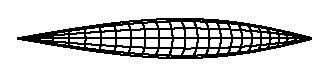
\includegraphics{asy/sin-mini}
\vskip-0mm
\end{Figure}

По \ref{ex:rev(sin)} гауссова кривизна поверхности вращения графика $y=a\cdot \sin x$ для $x\in(0,\pi)$ не может превышать $1$.
Попробуйте подпереть поверхность $\Sigma$ изнутри поверхностью вращения указанного типа.
(Сравните с \ref{ex:convex small}.)

\parit{Замечание.}
Упражнение можно вывести из следующего более глубокого результата: \textit{если гауссова кривизна замкнутой поверхности $\Sigma$ не меньше $1$,
то внутренний диаметр $\Sigma$ не больше $\pi$}.
Это означает, что любые две точки на $\Sigma$ можно соединить путём на $\Sigma$, длины не более~$\pi$.
Эту теорему доказали Хайнц Хопф и Вилли Ринов \cite{hopf-rinow} и она названа в честь, обобщившего её, Самнера Майерса \cite{myers}.

\parbf{\ref{ex:convex-proper-sphere}}; \ref{SHORT.ex:convex-proper-sphere:single}.
Воспользуйтесь выпуклостью~$R$.

\parit{\ref{SHORT.ex:convex-proper-sphere:smooth}.}
Обратите внимание, что отображение $\Sigma\to\mathbb{S}^2$ гладкое и регулярное.
Затем, применив теорему об обратной функции, покажите, что его обратное отображение также гладко.

\begin{wrapfigure}{r}{29 mm}
\vskip-4mm
\centering
\includegraphics{mppics/pic-1182}
\vskip-3mm
\end{wrapfigure}

\parbf{\ref{ex:convex-proper-plane}}; \ref{SHORT.ex:convex-proper-plane:a}
(Рассуждение похоже на \ref{prop:convex-monotone:open}.)
Можно предположить, что начало координат лежит на~$\Sigma$.
Рассмотрим последовательность точек $x_n\in \Sigma$, таких что $|x_n|\z\to \infty$ при $n\to \infty$.
Обозначим через $\vec u_n$ единичный вектор в направлении $x_n$; то есть $\vec u_n\z=\tfrac{x_n}{|x_n|}$.

Поскольку единичная сфера компактна, найдётся подпоследовательность $x_n$, такая что $\vec u_n$ сходится к единичному вектору, скажем к $\vec u$.
Покажите, что луч из начала координат в направлении $\vec u$ можно взять за~$\ell$.

\parit{\ref{SHORT.ex:convex-proper-plane:b} $+$ \ref{SHORT.ex:convex-proper-plane:c} $+$ \ref{SHORT.ex:convex-proper-plane:d}.}
Так как $R$ выпукло, то выпукла и его проекция $\Omega$.

Убедитесь, что для любого $q\in \Sigma$ направления $\vec v_n=\tfrac{x_n-q}{|x_n-q|}$ также сходятся к $\vec u$, и воспользуйтесь этим.

Покажите, что у $\Sigma$ нет вертикальных касательных плоскостей.
Выведите отсюда, что проекция из $\Sigma$ на $(x,y)$-плоскость регулярна.
Воспользовавшись теоремой об обратной функции, покажите, что множество $\Omega$ открыто.

\parit{\ref{SHORT.ex:convex-proper-plane:e}.}
Рассуждая от противного, допустим, что для некоторой последовательности $(x_n,y_n)\z\to(x_\infty,y_\infty)\in \partial\Omega$ последовательность $f(x_n,y_n)$ остаётся ограниченной сверху.
Тогда найдётся подпоследовательность, что $f(x_n,y_n)$ сходится к конечному значению, скажем $z_\infty$, либо расходится к $-\infty$.

В первом случае покажите, что точка $(x_\infty, y_\infty,z_\infty)$ не лежит на $\Sigma$, но имеет произвольно близкие точки на~$\Sigma$.
То есть $\Sigma$ не собственная --- противоречие.

Если $f(x_n,y_n)\to -\infty$, используйте выпуклость $f$, чтобы показать, что $f(\tfrac{x_n}2 ,\tfrac{y_n}2)\z\to -\infty$.
Заметьте, что начало координат принадлежит $\Omega$;
используйте это, чтобы показать, что $(\tfrac{x_\infty}2, \tfrac{y_\infty}2)\in\Omega$,
и придите к противоречию.

\parbf{\ref{ex:open+convex=plane}.}
Согласно \ref{ex:convex-proper-plane:d}, $\Sigma$ параметризуется открытой выпуклой областью $\Omega$ плоскости.
Остаётся показать, что $\Omega$-й можно запараметризовать всю плоскость.

Можно предположить, что начало координат плоскости лежит в $\Omega$.
Убедитесь, что в этом случае граница $\Omega$ записывается в полярных координатах как $(\theta,f(\theta))$, где $f\:\mathbb{S}^1\to\mathbb{R}$ --- положительная непрерывная функция.
Тогда гомеоморфизм из $\Omega$ на плоскость можно описать в полярных координатах, изменяя только радиальную координату;
например, как 
$(\theta,r)\z\mapsto (\theta,
\tfrac{r}{1-r/f(\theta)})$.

Во второй части воспользуйтесь \ref{ex:star-shaped-disc:nonsmooth}.

\parbf{\ref{ex:circular-cone}.}
Выберите координаты так, чтобы плоскость $(x,y)$ подпирала $\Sigma$ снизу в начале координат. 

Покажите, что для некоторого $\epsilon>0$ любая прямая, выходящая из начала координат под наклоном не больше $\epsilon$, может пересекать $\Sigma$ только в единичном шаре с центром в начале координат;
можно предположить, что $\epsilon$ мало, скажем $\epsilon<1$.
Рассмотрите конус, образованный лучами из начала координат под наклоном $\epsilon$ и сдвинутый вниз на $1$.
Убедитесь, что вся поверхность лежит внутри этого конуса.

\parbf{\ref{ex:intK}}.
Выберите различные точки $p,q\in\Sigma$.
Применив \ref{thm:convex-embedded}, покажите, что угол $\measuredangle(\Norm(p),p-q)$ острый, а $\measuredangle(\Norm(q),p-q)$ тупой.
Выведите отсюда, что $\Norm(p)\ne\Norm(q)$;
то есть отображение $\Norm\:\Sigma\to\mathbb{S}^2$ инъективно.

\parit{\ref{SHORT.ex:intK:4pi}.}
Для заданного единичного вектора $\vec u$ рассмотрим точку $p\in \Sigma$, которая максимизирует скалярное произведение $\langle p,\vec u\rangle$.
Покажите, что $\Norm(p)=\vec u$.
Выведите отсюда, что отображение $\Norm\:\Sigma\to\mathbb{S}^2$ сюръективно, и, следовательно, биективно.

Применив \ref{cor:intK}, получите, что наш интеграл равен $4\cdot\pi=\area\mathbb{S}^2$.

\parit{\ref{SHORT.ex:intK:2pi}.}
Выберите $(x,y,z)$-координаты, полученные в \ref{ex:convex-proper-plane:d}.
Убедитесь, что нормаль $\Norm(p)$ образует тупой угол с осью $z$ для любой точки~$p$.
Следовательно, образ $\Norm(\Sigma)$ лежит в южном полушарии.

Применив \ref{cor:intK}, получите, что наш интеграл не превосходит $2\cdot\pi=\tfrac12\cdot\area\mathbb{S}^2$.

\parit{Замечание.}
Это упражнение напоминает следствие~\ref{cor:fenchel=convex}.

\stepcounter{chapter}
\setcounter{eqtn}{0}

\parbf{\ref{ex:convex-revolution}.}
Примените \ref{ex:principal-revolution}.

\parbf{\ref{ex:ruled=>saddle}.}
Докажите, что каждая точка на поверхности имеет направление с нулевой нормальной кривизной, и воспользуйтесь этим.

\parbf{\ref{ex:saddle-convex}.}
Допустим, что $p\in \Sigma$ --- точка локального максимума~$f$.
Покажите, что $\Sigma$ подпирается своей касательной плоскостью в~$p$,
и придите к противоречию.

\parbf{\ref{ex:panov}.}
Пусть $\Pi_t$ --- аффинная касательная плоскость к $\Sigma$ в точке $\gamma(t)$, а через $\ell_t$ --- касательная прямая к $\gamma$ в момент времени~$t$.

Заметим, что $\Pi_t$ --- график функции, скажем, $h_t$, определённой на $(x, y)$-плоскости.
Обозначим через $\bar\ell_t$ проекцию $\ell_t$ на $(x, y)$-плоскость.
Покажите, что производная $\tfrac{d}{dt}h_t(w)$ обращается в ноль в точке $w$ тогда и только тогда, когда $w\in \bar\ell_t$, и эта производная меняет знак, если $w$ переходит с одной стороны $\bar\ell_t$ на другую.

Если $\bar\gamma$ звёздна относительно точки $w$, то $w$ не может пересечь $\bar\ell_t$.
Поэтому функция $t\mapsto h_t(w)$ монотонна на $\mathbb{S}^1$.
Убедитесь, что эта функция непостоянна, и придите к противоречию.

\parit{Источник:}
Это результат Дмитрия Панова~\cite{panov-curves}.

\parbf{\ref{ex:crosss}.}
Это частный случай так называемой \index{лемма Морса}\emph{леммы Морса}.
Мы приведём выжимку из её доказательства.
Более концептуальное доказательство \cite{abraham-marsden-ratiu} строится на трюке Мозера; см. решение упражнения \ref{ex:star-shaped-disc}.

\medskip

Выберите касательно-нормальные координаты при $p$ с координатными осями вдоль главных направлений.
Предположим, что $\Sigma$ локально задаётся графиком $z=f(x,y)$.
Надо показать, что решение $f(x,y)=0$ есть объединение двух гладких кривых, пересекающихся в $p$.

Докажите следующее утверждение:
\textit{Пусть $x\z\mapsto h(x)$ --- гладкая функция, определённая в открытом интервале $\mathbb{I}\ni0$, такая что $h(0)=h'(0)=0$ и $h''(0)>0$.
Тогда, на меньшем интервале $\mathbb{J}\ni0$ существует единственная гладкая функция $a\:\mathbb{J}\to\mathbb{R}$ такая, что $h=a^2$, $a(0)=0$ и $a'(0)> 0$.}

Заметьте, что, сузив область до малого квадрата  $|x|,|y|<\epsilon$, можно считать, что $f_{xx}\z>\epsilon$ и $f_{yy}<-\epsilon$.
Покажите, что если $\epsilon$ мало, то для каждого $x$ существует единственное $y(x)$ такое, что $f_x(x,y(x))=0$; более того, функция $x\z\mapsto y(x)$ является гладкой.

Пусть $h(x)=f(x,y(x))$.
Убедитесь, что $h(0)\z=h'(0)=0$ и $h''>0$.
Применив утверждение выше, получите такую функцию $a$, что $h=a^2$, где $a(0)=0$ и $a'(0)>0$.

Убедитесь, что $g(x,y)=h(x)-f(x,y)\z\ge 0$, $g_y(x,y(x))\z=g(x,y(x))\z=0$, и $g_{yy}>0$.
Применяя утверждение к каждой функции $y\mapsto g(x,y)$ с фиксированным $x$, мы получаем, что $g(x,y)=b(x,y)^2$ для некоторой гладкой функции $b$, такой что 
$b(x,y(x))=0$ и $b_y(x,y(x))>0$.

Отсюда следует, что 
\begin{align*}
f(x,y)&=a(x)^2-b(x,y)^2=
\\
&=
(a(x)-b(x,y))\cdot (a(x)+b(x,y)).
\end{align*}
То есть $f(x,y)=0$ значит, что $a(x)=\pm b(x,y)$.

Остаётся проверить, что обе функции $g_\pm(x,y)=a(x)\pm b(x,y)$ имеют различные ненулевые градиенты в нуле, и, значит, каждое уравнение $a(x)\pm b(x,y) =0$ определяет гладкую кривую в окрестности $p$;
см.~\ref{sec:implicit-curves}.

\parbf{\ref{ex:proper-saddle}.}
Посмотрите на псевдосферу в \ref{ex:principal-revolution:pseudosphere}.

\parbf{\ref{ex:length-of-bry}.}
Воспользуйтесь \ref{lem:convex-saddle} и леммой о полусфере (\ref{lem:hemisphere}).

Во второй части постройте тонкую трубку, ограниченную двумя замкнутыми сферическими кривыми.

\parbf{\ref{ex:circular-cone-saddle}.}
Пусть $\Sigma$ --- открытая седловая поверхность, лежащая в конусе $K$.
Покажите, что существует плоскость $\Pi$, которая пересекает $\Sigma$ и отсекает от $K$ компактную область.
Выведите отсюда, что $\Pi$ также отсекает от $\Sigma$ компактную область.

Воспользовавшись \ref{lem:reg-section}, сдвиньте немного плоскость $\Pi$ так, чтобы она отсекала от $\Sigma$ компактную поверхность с границей, и примените \ref{lem:convex-saddle}.

\parbf{\ref{ex:disc-hat}.}
Рассмотрим радиальную проекцию $F_\epsilon$ на сферу $\Sigma$ с центром в точке $p=(0,0,\epsilon)$;
то есть точка $q\in F_\epsilon$ переходит в точку $s(q)$ на сфере, лежащую на луче $pq$.

Покажите, что $s$ задаёт диффеоморфизм из $F_\epsilon$ на южную полусферу в~$\Sigma$.
Остаётся заметить, что единичный диск диффеоморфен полусфере.

\parbf{\ref{ex:saddle-linear}.} 
По основной теореме аффинной геометрии, аффинное преобразование является гладким.
Остаётся применить критерий горбушек (\ref{prop:hat}).

\parbf{\ref{ex:between-parallels}.}
Поищите пример среди поверхностей вращения;
воспользуйтесь \ref{ex:principal-revolution}.

\parbf{\ref{ex:one-side-bernshtein}.}
Рассмотрите сечения графика плоскостями, параллельными плоскостям $(x,y)$ и $(x,z)$, и примените теорему Мёнье (\ref{thm:meusnier}).

\parbf{\ref{ex:saddle-graph}.}
Допустим, что ортогональная проекция $\Sigma$ на $(x,y)$-плоскость не инъективна.
Покажите, что существует точка $p\in\Sigma$ с вертикальной касательной плоскостью;
то есть $\T_p\Sigma$ перпендикулярна плоскости $(x,y)$.

Пусть $\Gamma_p$ --- связная компонента точки $p$ в пересечении $\Sigma$ с аффинной касательной плоскостью $\T_p\Sigma$.
Воспользовавшись \ref{ex:crosss}, покажите, что $\Gamma_p$ представляет собой объединение гладких кривых, которые могут пересекаться друг с другом трансверсально.
Более того, две из этих кривых проходят через $p$, и $\Gamma_p$ не ограничивает компактную область на~$\Sigma$.

Покажите, что у множества $\Gamma_p$ должно быть как минимум 4 направления, в которых оно уходит на бесконечность.
С другой стороны, $\Sigma$ является графиком вне компактного множества $K$.
Значит, $\Gamma_p\setminus K$ --- график вещественной функции одной переменной, который имеет только два направления, в которых он уходит на бесконечность --- противоречие.

%\end{multicols}
%\par\noindent\rule{\textwidth}{0.4pt}
%\begin{multicols}{2}

\stepcounter{chapter}
\setcounter{eqtn}{0}

\begin{wrapfigure}{r}{24 mm}
\vskip-4mm
\centering
\includegraphics{mppics/pic-1250}
\vskip-0mm
\end{wrapfigure}

\parbf{\ref{ex:lasso}.}
Разрежьте боковую поверхность горы по отрезку от ковбоя до вершины и
разверните её на плоскости (см. рисунок).
Подумайте, как может выглядеть образ натянутого лассо.

\parit{Источник:}
Эту задачу мы узнали от Джоэля Файна, который приписывает её Фредерику Буржуа \cite{fine}.

\parbf{\ref{ex:length-dist-conv}.} 
Согласно \ref{thm:convex-embedded}, $\Sigma$ ограничивает строго выпуклую область.
Поэтому можно предположить, что $\Norm(p)\ne\Norm(q)$; в противном случае, $p=q$, и неравенство очевидно.

Ещё можно предположить, что $\Norm(p)\z+\Norm(q)\z\ne 0$; в противном случае, правая часть неопределена.

В оставшемся случае касательные плоскости $\T_p$ и $\T_q$ пересекаются по прямой, скажем, $\ell$.
Положим $\alpha=\tfrac12\cdot\measuredangle(\Norm(p),\Norm(q))$.
Убедитесь, что $2\cdot\cos\alpha\z= |\Norm(p)+\Norm(q)|$.
Пусть точка $x\in \ell$ минимизирует сумму $|p-x|\z+|x-q|$.
Покажите, что $\measuredangle\hinge xpq\ge \pi-2\cdot\alpha$.
Выведите отсюда, что 
\[
|p-x|+|x-q|\le \tfrac{|p-q|}{\cos\alpha}.
\]
Применив \ref{thm:shorts+convex}, покажите, что
$\dist{p}{q}\Sigma\z\le |p-x|+|x-q|$.

\parbf{\ref{ex:hat-convex}.}
Допустим, что нашлась кратчайшая $\gamma\not\subset\Delta$ с концами $p$ и $q$ в $\Delta$.

Можно предположить, что только одна дуга $\gamma$ лежит вне $\Delta$.
Отражение этой дуги относительно $\Pi$ вместе с оставшейся частью $\gamma$ образует другую кривую $\hat\gamma$ из $p$ в $q$;
часть её идёт по $\Sigma$, 
а часть снаружи $\Sigma$,
но она никогда не заходит внутрь.
Заметьте, что
\[\length\hat\gamma=\length\gamma.\]

Обозначим через $\bar\gamma$ ближайшую проекцию точки $\hat\gamma$ на~$\Sigma$.
Кривая $\bar\gamma$ лежит в $\Sigma$, 
имеет те же концы, что и $\gamma$,
и по \ref{thm:shorts+convex}
\[\length\bar\gamma<\length\gamma.\]
Это означает, что $\gamma$ не была кратчайшей --- 
противоречие.

\parbf{\ref{ex:intrinsic-diameter}.} 
Докажите, что короткая проекция $\mathbb{S}^2\to\Sigma$ сюръективна.
Примените \ref{lem:nearest-point-projection} и \ref{thm:area-axioms:monotonicity}.

%\end{multicols}
%\par\noindent\rule{\textwidth}{0.4pt}
%\begin{multicols}{2}

\stepcounter{chapter}
\setcounter{eqtn}{0}

\parbf{\ref{ex:helix-geodesic}.}
Докажите, что $\gamma''(t)$ пропорциональна $\nabla_{\gamma(t)} f$, где $f=x^2+y^2$. 
Примените \ref{ex:tangent-normal}.

\parbf{\ref{ex:clairaut}.} 
Мы можем предположить, что начало координат лежит на оси вращения, а вектор $\vec i$ направлен вдоль этой оси.
Воспользовавшись \ref{lem:constant-speed}, покажите, что достаточно доказать, что 
значение $\langle\gamma'\times \gamma,\vec i\rangle$ постоянно.

Поскольку $\gamma''(t)\perp\T_{\gamma(t)}$, три вектора $\vec i$, $\gamma$, и $\gamma''$ лежат в одной плоскости.
В частности, $\langle\gamma''\times \gamma,\vec i\rangle=0$.
Следовательно,
\[
\langle\gamma'\times \gamma,\vec i\rangle'
=
\langle\gamma'\times \gamma',\vec i\rangle+\langle\gamma''\times \gamma,\vec i\rangle =0
.\]

\parbf{\ref{ex:asymptotic-geodesic}.}
По лемме \ref{lem:constant-speed}, можно считать, что $\gamma$ параметризована длиной.
По определению геодезической, $\gamma''(s)\perp\T_{\gamma(s)}$. 
Следовательно, 
\[\gamma''(s)=k_n(s)\cdot\Norm(\gamma(s)),\]
где $k_n(s)$ --- нормальная кривизна кривой $\gamma$ в момент времени $s$.
Поскольку $\gamma$ --- асимптотическая линия, $k_n(s)\equiv 0$;
то есть $\gamma''(s)\equiv 0$.
Следовательно, $\gamma'$ постоянна, и, значит, $\gamma$ идёт вдоль прямой; см. \ref{ex:zero-curvature-curve}.

\parbf{\ref{ex:reflection-geodesic}.}
Обозначим через $\mu$ единичный вектор, перпендикулярный плоскости симметрии $\Pi$.
Раз уж $\gamma$ лежит в $\Pi$, её ускорение $\gamma''$ направлено вдоль $\Pi$, иначе говоря, $\gamma''\perp \mu$.
Из \ref{prop:a'-pertp-a''}, $\gamma''\perp\gamma'$, ведь $\gamma$ параметризована длиной.

Поскольку $\Sigma$ симметрична относительно плоскости $\Pi$,
касательная плоскость $\T_{\gamma(t)}\Sigma$ также симметрична относительно $\Pi$.
Отсюда вытекает, что $\T_{\gamma(t)}\Sigma$ натянута на $\mu$ и $\gamma'(t)$.
Следовательно, $\gamma''\perp \mu$ и $\gamma''\perp\gamma'$ подразумевают $\gamma''\perp\T_{\gamma(t)}\Sigma$;
то есть $\gamma$ является геодезической.

\parbf{\ref{ex:round-torus}.}
Согласно \ref{ex:reflection-geodesic}, любой меридиан $\Sigma$ является замкнутой геодезической.
Рассмотрим произвольную замкнутую геодезическую~$\gamma$.

Если $\gamma$ касается меридиана в какой-то точке, то по единственности в \ref{prop:geod-existence}, кривая $\gamma$ идёт вдоль этого меридиана;
в частности, она не стягиваема.

В оставшемся случае $\gamma$ может пересекать меридианы только трансверсально.
Следовательно, долгота $\gamma$ монотонна, и снова $\gamma$ не стягиваема.

\parbf{\ref{ex:helix=geodesic}.}
Проверьте, что $\Norm(\gamma(t))\z=(\cos t,\sin t, 0)$.
Далее, вычислите ускорение $\gamma''(t)$ и убедитесь, что оно пропорционально $\Norm(\gamma(t))$,
а значит, $\gamma''(t)\z\perp\T_{\gamma(t)}$. 

Убедитесь, что отрезок от $\gamma (0)$ до $\gamma (2{\cdot}\pi)$ содержится в~$\Sigma$,
и воспользуйтесь этим.

\parbf{\ref{ex:two-min-geod}.}
Допустим, что две кратчайшие $\alpha$ и $\beta$ имеют пару общих точек $p$ и~$q$.
Обозначим через $\alpha_1$ и $\beta_1$ дуги $\alpha$ и $\beta$ от $p$ до~$q$.
Предположим, что $\alpha_1$ не совпадает с $\beta_1$.

Заметьте, что $\alpha_1$ и $\beta_1$ --- кратчайшие с теми же концами;
в частности, они одинаковой длины.
Замена $\alpha_1$ в $\alpha$ на $\beta_1$ даёт кратчайшую, скажем, $\hat\alpha$, отличную от $\alpha$.
По \ref{prop:gamma''}, $\hat\alpha$ --- геодезическая.

\begin{Figure}
\vskip-0mm
\centering
\includegraphics{mppics/pic-308}
\vskip0mm
\end{Figure}

Предположим, что $\alpha_1$ --- собственная поддуга $\alpha$;
то есть $\alpha_1\ne\alpha$, иначе говоря, $p$ или $q$ не конец кривой $\alpha$.
Тогда у $\alpha$ и $\hat\alpha$ есть общая точка и общий вектор скорости в этой точке.
По \ref{prop:geod-existence}, $\alpha$ совпадает с $\hat\alpha$ --- противоречие.

Следовательно, $p$ и $q$ --- концы~$\alpha$.
Аналогично, $p$ и $q$ --- концы~$\beta$.

Для второй части можно рассмотреть две различные геодезические вида 
\[ \gamma_b(t) = ( \cos t , \sin t , b\cdot t ) , t \in \mathbb{R} \]
на цилиндрической поверхности $x^2 + y^2 =1$.

\parbf{\ref{ex:min-geod+plane}.}
Допустим, что кратчайшая $\alpha$ проходит сквозь $\Pi$ два раза или больше.
В этом случае найдётся дуга $\alpha_1$ в $\alpha$, которая лежит строго на одной стороне от $\Pi$, только её концы лежат на $\Pi$, и эти концы отличаются от концов $\alpha$.

\begin{Figure}
\vskip-1mm
\centering
\includegraphics{mppics/pic-310}
\vskip-1mm
\end{Figure}

Удалим из $\alpha$ дугу $\alpha_1$ и заменим её отражением $\alpha_1$ в $\Pi$.
Полученная кривая, назовём её $\beta$, лежит на поверхности;
она имеет ту же длину, что и $\alpha$, и соединяет ту же пару точек, скажем, $p$ и~$q$.
Следовательно, $\beta$ --- это кратчайшая от $p$ до $q$ на $\Sigma$, отличная от~$\alpha$.

Мы можем предположить, что и $\alpha$, и $\beta$ параметризованы длиной.
По \ref{prop:gamma''}, $\alpha$ и $\beta$ --- геодезические.
Поскольку $\alpha$ и $\beta$ имеют общую дугу, у них есть общая точка и общий вектор скорости в этой точке;
по \ref{prop:geod-existence} $\alpha$ совпадает с $\beta$ --- противоречие.

\parbf{\ref{ex:milka}.}
Пусть $W$ --- замкнутая область снаружи~$\Sigma$.
Убедитесь, что $\dist{p^s}{q}W$ не зависит от~$s$.
Иначе говоря, произведение отрезка $[p^s,\gamma(s)]$ и дуги $\gamma|_{[s,\ell]}$ есть кратчайшая от $p^s$ до $q$ в~$W$.

Так как $\Sigma$ строго выпукла, 
\[ \dist{\gamma (s)}{q}W > \dist{\gamma(s)}{q}{\mathbb{R}^3} \]
для всех $s < \ell$.
Следовательно,
\begin{align*}
\dist{p^s}{q}W&=\dist{p^s}{\gamma(s)}W+\dist{\gamma (s)}{q}W 
> 
\\
&>\dist{p^s}{\gamma(s)}{\mathbb{R}^3} + \dist{ \gamma (s)}{q}{\mathbb{R}^3} 
\ge
\\
&\ge\dist{p^s}{q}{\mathbb{R}^3}. 
\end{align*}
Однако, если отрезок $[p^s,q]$ целиком содержится в $W$, то $\dist{p^s}{q}W = \dist{p^s}{q}{\mathbb{R}^3}$, и это приводит к противоречию.

\parbf{\ref{ex:round-sphere}.}
Рассуждая как в \ref{ex:const-dist}, докажите, что все геодезические на поверхности  имеют постоянную кривизну.
Выведите отсюда, все нормальные кривизны поверхности равны между собой, и рассуждайте как в \ref{ex:normal-curvature=const}.

\parit{Источник:} Задача Али Тагави \cite{taghavi}.

\parbf{\ref{ex:closed-liberman}.}
Пусть $t\mapsto \gamma(t)=(x(t),y(t),z(t))$ --- замкнутая геодезическая с единичной скоростью на графике $z=f(x,y)$.
По лемме Либермана, функция $t\mapsto z'(t)$ монотонна.
Выведите отсюда, что координата $z$ постоянна на $\gamma$, то есть $\gamma$ лежит в горизонтальной плоскости.
Докажите, что $\gamma$ --- прямая, и придите к противоречию.

\parbf{\ref{ex:rho''}.}
Снабдите $\Sigma$ полем нормалей $\Norm$, направленным внутрь.
Обозначим через $k(t)$ нормальную кривизну $\Sigma$ в точке $\gamma(t)$ в направлении $\gamma'(t)$.
Поскольку $\Sigma$ выпукла, $k(t)\ge 0$ для любого~$t$.

Поскольку $\gamma$ --- геодезическая с единичной скоростью, $\gamma''(t)=k(t)\cdot\Norm(\gamma(t))$ и $\langle\gamma'(t),\gamma'(t)\rangle=1$ для любого~$t$.
Можно предположить, что $p$ --- начало координат в~$\mathbb{R}^3$.
Поскольку $p$ находится внутри $\Sigma$, получаем, что $\langle\gamma(t),\Norm(\gamma(t))\rangle\le 0$ и
\[
\langle\gamma''(t),\gamma(t)\rangle=k(t)\cdot \langle\gamma(t),\Norm(\gamma(t))\rangle\le 0
\]
для любого~$t$.
Выведите отсюда, что
\begin{align*}
&\rho''(t)
=\langle\gamma(t),\gamma(t)\rangle''=
\\
&=2\cdot\langle\gamma''(t),\gamma(t)\rangle+2\cdot\langle\gamma'(t),\gamma'(t)\rangle\le 2.
\end{align*}

\parbf{\ref{ex:tc-spherical-image}.}  
Можно считать, что $\gamma$ параметризована длиной.
Определим $\Norm (t) \df \Norm ( \gamma (t))$.
Тогда $\langle \gamma'(t), \Norm(t) \rangle \equiv 0$,
и поскольку $\gamma$ геодезическая, $\gamma''(t) \parallel \Norm (t)$.
Отсюда
\[
\begin{aligned}
|\gamma''(t)|
&=|\langle\gamma''(t),\Norm(t)\rangle|=
\\
&=|\langle\gamma'(t),\Norm(t)\rangle'-\langle\gamma'(t),\Norm'(t)\rangle|=
\\
&=|\langle\gamma'(t),\Norm'(t)\rangle|\le
\\
&\le|\gamma'(t)|\cdot|\Norm'(t)|=|\Norm'(t)|.
\end{aligned}
\]
Проинтегрируйте по $t$ и получите 
\[\tc\gamma\le\length(\Norm\circ\gamma).\]

\parbf{\ref{ex:usov-exact}.} 
Пусть $\gamma(t)=(x(t),y(t),z(t))$. 
Покажите, что
\[
|\gamma'' (t)| = z''(t)\cdot\sqrt{1+ \ell ^2}\eqlbl{eq:gamma''=z''}
\]
для любого~$t$.

Убедитесь, что $z'(t)\to\pm \tfrac\ell{\sqrt{1+ \ell ^2}}$ при $t\z\to\pm\infty$.
Выведите отсюда, что 
\[
\int_{-\infty}^{+\infty}z''(t)\cdot dt
=
\frac{2\cdot\ell}{\sqrt{1+ \ell ^2}}.\eqlbl{eq:int z''}
\]
Из \ref{eq:gamma''=z''} и \ref{eq:int z''},
\begin{align*}
\tc\gamma&=\int_{-\infty}^{+\infty}|\gamma''(t)|\cdot dt=
\\
&=
\sqrt{1+ \ell ^2}\cdot \int_{-\infty}^{+\infty}z''(t)\cdot dt=
\\
&=2\cdot \ell.
\end{align*}

\parbf{\ref{ex:ruf-bound-mountain}.}
Воспользуйтесь \ref{thm:usov} и \ref{ex:sef-intersection}.

Во второй части рассмотрите геодезическую на конусе с угловым коэффициентом $2$, и сгладьте его вершину.

\parit{Замечание.}
Утверждение остаётся верным для $\sqrt{3}$-липшицевых функций, и $\sqrt{3}=\tg\tfrac\pi3$ --- оптимальная константа; см. \ref{ex:sqrt(3)}.
Это тот же угловой коэффициент, что и в задаче про ковбоя и лассо (\ref{ex:lasso}).

\parbf{\ref{ex:bound-tc}}; \ref{SHORT.ex:bound-tc:a}.
Убедитесь, что 
\[|\gamma|\le 1
\qquad
\text{и}
\qquad
\langle\Norm,\epsilon\cdot \Norm-\gamma\rangle\le0,\]
и воспользуйтесь этим.

\parit{\ref{SHORT.ex:bound-tc:b}.}
Покажите, что  
\[|\gamma|\le 1,\quad |\gamma'|= 1
\quad
\text{и}
\quad \rho'=2\cdot \langle\gamma,\gamma'\rangle,\]
и воспользуйтесь этим.

\parit{\ref{SHORT.ex:bound-tc:c}.}
Покажите, что
\begin{align*}
|\gamma'|&= 1,
&
\langle\gamma,\Norm\rangle&=|\gamma|\cdot\cos\theta,
\\
\gamma''&=-k\cdot \Norm,
&
\rho''&=2\cdot \langle\gamma',\gamma'\rangle+2\cdot \langle\gamma,\gamma''\rangle,
\end{align*}
и воспользуйтесь этим.

\parit{\ref{SHORT.ex:bound-tc:d}.}
Пусть $x,y$ --- точки на единичной сфере, проектирующиеся в концы $\gamma$. 
Соедините $x$ с $y$ дугой длины $\le \pi$ на сфере, спроектируйте её на $\Sigma$.
Примените \ref{lem:nearest-point-projection} и воспользуйтесь тем, что $\gamma$ --- кратчайшая.

\parit{\ref{SHORT.ex:bound-tc:e}.}
Пусть $\gamma\:[0,\ell]\to\Sigma$ --- параметризация длиной.
Воспользовавшись \ref{SHORT.ex:bound-tc:d}, покажите, что $\ell\le \pi$.
Воспользовавшись \ref{SHORT.ex:bound-tc:a}, \ref{SHORT.ex:bound-tc:b}, \ref{SHORT.ex:bound-tc:c} и тем, что $|\gamma|\ge \epsilon$, выведите, что 
\[2\cdot \ell-2\cdot \epsilon^2\cdot \tc{\gamma}
\ge
\int_0^\ell\rho''(t)\cdot dt.\]
Из \ref{SHORT.ex:bound-tc:b} выведите, что $\int\rho''\ge -4$.
Сделайте последний шаг.

%\end{multicols}
%\par\noindent\rule{\textwidth}{0.4pt}
%\begin{multicols}{2}
 
\stepcounter{chapter}
\setcounter{eqtn}{0}

\parbf{\ref{ex:parallel}}; \ref{SHORT.ex:parallel:a}.
Покажите, что $\langle\vec v(t),\vec v'(t)\rangle=0$, и воспользуйтесь этим.

\parit{\ref{SHORT.ex:parallel:b}}
Покажите, что $|\vec v(t)|$, $|\vec w(t)|$, и
$\langle\vec v(t),\vec w(t)\rangle$
не меняются; это можно сделать так же, как в \ref{SHORT.ex:parallel:a}.
Затем воспользуйтесь тем, что 
$\langle\vec v(t),\vec w(t)\rangle\z=|\vec v(t)|\cdot|\vec w(t)|\cdot\cos\theta$.

\parbf{\ref{ex:parallel-transport-support}.}
Заметьте, что $\Sigma_1$ подпирает $\Sigma_2$ в каждой точке кривой~$\gamma$.
Выведите отсюда, что у $\gamma$ как кривой на $\Sigma_1$ и на $\Sigma_2$ идентичные нормали.
Примените \ref{obs:parallel=}.

\parbf{\ref{ex:holonomy=not0}.}
Почти любая замкнутая кривая решает задачу.
Например, рассмотрите прямоугольный сферический треугольник, который вырезается октантом $\mathbb{R}^3$ из сферы.
Покажите, что параллельный перенос вокруг него поворачивает касательную плоскость на угол $\tfrac\pi 2$.

\stepcounter{chapter}
\setcounter{eqtn}{0}

\parbf{\ref{ex:1=geodesic-curvature}.}
По \ref{ex:convex-proper-sphere}, $\Sigma$ --- гладкая сфера.
По теореме Жордана (\ref{thm:jordan}), кривая $\gamma$ делит $\Sigma$ на два диска.
Обозначим через $\Delta$ диск, который лежит слева от~$\gamma$.

Убедитесь, что $\tgc\gamma=\length\gamma$, и примените формулу Гаусса --- Бонне (\ref{thm:gb}) к~$\Delta$.

\parbf{\ref{ex:GB-hat}.}
Покажите, что $\skur=\cos\alpha\cdot\skur_0$,
где $\skur$ --- геодезическая кривизна $\partial \Delta$ в $\Delta$,
а $\skur_0$ --- геодезическая кривизна $\partial \Delta$ в $(x,y)$-плоскости.
Примените \ref{prop:total-signed-curvature} и формулу Гаусса --- Бонне (\ref{thm:gb}).

\parbf{\ref{ex:geodesic-half}.}
Воспользуйтесь \ref{cor:intK}, \ref{ex:intK:4pi} и формулой Гаусса --- Бонне (\ref{thm:gb}).

В последней части примените \ref{ex:bisection-of-S2}.

\parbf{\ref{ex:closed-geodesic}.}
В первой части примените формулу Гаусса --- Бонне (\ref{thm:gb}).

Во второй части, если бы две замкнутые геодезические $\gamma_1$ и $\gamma_2$ не пересекались, то 
$\gamma_2$ лежала бы в одной из областей, скажем $R_1$, которую $\gamma_1$ вырезает из~$\Sigma$.
Аналогично, $\gamma_1$ лежала бы в одной из областей, скажем $R_2$, которую $\gamma_2$ вырезает из~$\Sigma$.

Заметьте, что $R_1$ и $R_2$ покрывают $\Sigma$ с перекрытием.
Из первой части получаем, что интеграл гауссовой кривизны по $\Sigma$ строго меньше $4\cdot\pi$, а это противоречит \ref{ex:intK:4pi}.

\parbf{\ref{ex:self-intersections}}; \textit{(легкая)}.
Рассмотрите 4 области, ограниченные петлями.
Применив формулу Гаусса --- Бонне (\ref{thm:gb}), покажите, что интеграл гауссовой кривизны по каждой из этих областей превышает $\pi$.
Придите к противоречию с \ref{ex:intK:4pi}.

\parit{(сложная)}.
Пусть $\alpha$, $\beta$ и $\gamma$ --- углы треугольника.
Применив формулу Гаусса --- Бонне (\ref{thm:gb}), покажите, что три петли окружают области, на которых интеграл гауссовой кривизны равен $\pi+\alpha$, $\pi+\beta$ и $\pi+\gamma$.

Применив формулу Гаусса --- Бонне к треугольной области, убедитесь, что $\alpha+\beta\z+\gamma>\pi$.
Воспользуйтесь \ref{ex:intK:4pi} и придите к противоречию.

\parit{(безнадёжная)}.
Это правда сложно.
Решение на основе \ref{thm:comp:toponogov} приведено в \cite{petrunin2021}.

\parbf{\ref{ex:sqrt(3)}.}
Достаточно показать, что на поверхности нет геодезических петель.
Допустим нашлась петля, оцените интегралы гауссовой кривизны по всей поверхности и по диску, окружённому геодезической петлёй.

\parbf{\ref{ex:unique-geod}}; \ref{SHORT.ex:unique-geod:unique}.
Из \ref{prop:shortest-paths-exist} и \ref{prop:gamma''} вытекает, что любые две точки на $\Sigma$ можно соединить геодезической.
Допустим, что точки $p$ и $q$ можно соединить двумя различными геодезическими $\gamma_1$ и $\gamma_2$.
Перейдя к их дугам, можно считать, что у $\gamma_1$ и $\gamma_2$ нет общих точек кроме концов.
Поскольку поверхность односвязна, $\gamma_1$ и $\gamma_2$ вместе ограничивают диск, скажем, $\Delta\subset\Sigma$.
Остаётся применить формулу Гаусса --- Бонне к $\Delta$ и сделать вывод.

\parit{\ref{SHORT.ex:unique-geod:diffeomorphism}.} 
Воспользуйтесь частью \ref{SHORT.ex:unique-geod:unique} и \ref{prop:inj-rad}.

\parbf{\ref{ex:half-sphere-total-curvature}.}
Примените \ref{prop:pt+tgc} и \ref{prop:area-of-spher-polygon}.

\parbf{\ref{ex:cohn-vossen}.}
Рассуждайте как в конце доказательства \ref{thm:cohn-vossen} для однопараметрического семейства геодезических $\gamma_\tau$, заданных условием $\gamma_\tau(0)=\alpha(\tau)$ и $\gamma'_\tau(0)=\alpha'(\tau)$.


\parbf{\ref{ex:g-b-chi}.}
Разбейте поверхность на диски, подсчитайте число рёбер, вершин и дисков в полученном разбиении.
Вычислите эйлерову характеристику и примените \ref{thm:GB-generalized}.
Для ленты Мёбиуса и пары штанов, воспользуйтесь тем что граничные кривые имеют нулевую геодезическую кривизну.
Для цилиндра, воспользуйтесь тем, что граничные кривые плоски и замкнуты и примените \ref{prop:total-signed-curvature}.    


%\end{multicols}
%\par\noindent\rule{\textwidth}{0.4pt}
%\begin{multicols}{2}

\stepcounter{chapter}
\setcounter{eqtn}{0}

\parbf{\ref{ex:semigeodesc-chart}.}
По лемме Гаусса (\ref{lem:palar-perp}), полярные координаты с началом в точке $q$ задают полугеодезические карты в близлежащих точках.
Таким образом, достаточно найти точку $q\ne p$ чтобы полярные координаты на $\Sigma$ с началом в $q$ покрывали $p$.
Согласно \ref{prop:exp}, подойдёт любая точка $q$ достаточно близкая к $p$.

\parbf{\ref{ex:inj-rad}}; \ref{SHORT.ex:inj-rad:sign}.
Обратите внимание, что ориентацию на $\Sigma$ можно выбрать так, что $b_r(0,\theta)\z=1$ для любого $\theta$.
После этого, можно считать, что $b(r,\theta)>0$ для всех малых $r>0$.

Допустим, что $b(r_1,\theta_1)<0$ при некоторой паре $(r_1,\theta_1)$, таких что $0<r_1<r_0$.
Убедитесь, что если $\theta_2$ достаточно близко к $\theta_1$, то радиальные кривые $r\z\mapsto b(r,\theta_1)$ и $r\z\mapsto b(r,\theta_2)$, определённые на интервале $(0,r_1)$, пересекаются.
Следовательно, $\exp_p$ не является инъективным в $B$ --- противоречие.

\parit{\ref{SHORT.ex:inj-rad:0}.}
Допустим, что $b(r_1,\theta_1)=0$.
Примените \ref{SHORT.ex:inj-rad:sign}, чтобы показать, что $b_r(r_1,\theta_1)=0$.

Применив \ref{prop:jaccobi}, введите, что $b(r,\theta_1)=0$ для любого $r$.
Это противоречит тому, что $b_r(0,\theta_1)=1$.

\parit{\ref{SHORT.ex:inj-rad:prop:inj-rad}.}
Нужно показать, что $\exp_p$ регулярно в $B$.
Предположим, что вектор $\vec v\in B$ имеет полярные координаты $(r,\theta)$ для некоторого $r>0$.
Покажите, что $\exp_p$ регулярно в точке $\vec v$, если $b(r,\theta)\ne 0$.
Выведите, что $\exp_p$ регулярно в $B\setminus \{0\}$.

По \ref{obs:d(exp)=1}, $\exp_p$ регулярно в нуле.
Значит сужение $\exp_p|_B$ --- регулярное инъективное гладкое отображение.
Воспользовавшись теоремой об обратной функции (\ref{thm:inverse}), покажите, что сужение $\exp_p|_B$ есть диффеоморфизм на свой образ.


\parbf{\ref{lem:K(orthogonal)}}; \ref{SHORT.lem:K(orthogonal):uu-vv}.
Так как базис $\vec u, \vec v,\Norm$ ортонормирован,
первые два векторных тождества эквивалентны следующим шести вещественным:
\[
\begin{aligned}
\langle\vec u_u,\vec u\rangle
&=0,
&
\langle\vec v_u,\vec v\rangle
&=0,
\\
\langle\vec u_u,\vec v\rangle
&=-\tfrac1{b}\cdot a_v,
&
\langle\vec v_u,\vec u\rangle
&=
\tfrac1{b}\cdot a_v,
\\
\langle\vec u_u,\Norm\rangle
&=a\cdot \ell,
&
\langle\vec v_u,\Norm\rangle
&=
a\cdot m.
\end{aligned}
\eqlbl{eq:key-orthogonal/2}
\]

Взяв частные производные от тождеств
$\langle\vec u,\vec u\rangle=1$ и
$\langle\vec v,\vec v\rangle=1$ по $u$,
мы получаем первые два тождества в \ref{eq:key-orthogonal/2}.

Кроме того, заметим, что
\[
\begin{aligned}
\vec v_u
&=
\tfrac{\partial}{\partial v}
(\tfrac1b\cdot s_v)=\tfrac1b\cdot s_{uv}
+
\tfrac{\partial}{\partial u}(\tfrac1b)
\cdot
 s_v.
\end{aligned}
\eqlbl{eq:dv/du}
\]
Так как $s_u\perp s_v$, получаем, что
\begin{align*}
\langle\vec v_u,\vec u\rangle
&=
\tfrac1{a\cdot b}\cdot \langle s_{vu}, s_u\rangle=
\\
&=
\tfrac1{2\cdot a\cdot b}\cdot \tfrac{\partial}{\partial v}\langle s_u, s_u\rangle=
\\
&=
\tfrac1{2\cdot a\cdot b}\cdot \tfrac{\partial a^2}{\partial v}=
\\
&=
\tfrac1{b}\cdot a_v.
\end{align*}
Взяв частную производную $\langle\vec u,\vec v\rangle=0$ по $u$, получаем
\begin{align*}
\langle\vec v_u,\vec u\rangle+
\langle\vec v,\vec u_u\rangle
&=0.
\end{align*}
Получаем ещё пару тождеств из \ref{eq:key-orthogonal/2}.

Так как $\vec u$ и $\vec v$ ортонормированы, из \ref{thm:shape-chart} следует, что
\[
\begin{aligned}
\tfrac1{a^2}
\cdot
\langle s_{uu},\Norm\rangle
&=\ell,
&
\tfrac1{a\cdot b}
\cdot
\langle s_{uv},\Norm\rangle
&=m,
\\
\tfrac1{a\cdot b}
\cdot
\langle s_{vu},\Norm\rangle
&=m,
&
\tfrac1{b^2}
\cdot
\langle s_{vv},\Norm\rangle
&=n.
\end{aligned}
\eqlbl{eq:shape-lmn}
\]

Применив \ref{eq:dv/du}, \ref{eq:shape-lmn} и то, что $s_v\perp\Norm$, получаем
\begin{align*}
\langle\vec u_u,\Norm\rangle
&=
\tfrac1{a}\cdot \langle s_{uu},\Norm\rangle
=a\cdot \ell,
\\
\langle\vec v_u,\Norm\rangle
&=
\tfrac1{a}\cdot \langle s_{uv},\Norm\rangle
=a\cdot m.
\end{align*}
Мы получили последние два тождества в \ref{eq:key-orthogonal/2}.

Итак, мы доказали первые два тождества в \ref{SHORT.lem:K(orthogonal):uu-vv};
остальные доказываются также.

\parit{\ref{SHORT.lem:K(orthogonal):K}.}
Напомним, что гауссова кривизна равна определителю матрицы $
(\begin{smallmatrix}
\ell&m
\\
m&n
\end{smallmatrix}
)
$;
то есть $K=\ell\cdot n-m^2$.
Следовательно, 
\begin{align*}
a\cdot b\cdot K
&=
a\cdot b\cdot(\ell\cdot n-m^2)
=
\\
&=
\langle\vec u_u,\vec v_v\rangle 
-
\langle\vec u_v,\vec v_u\rangle= 
\\
&= 
\left(
\tfrac{\partial}{\partial v}
\langle\vec u_u,\vec v\rangle
-
\cancel{\langle\vec u_{uv},\vec v\rangle}
\right)-
\\
&-
\left(
\tfrac{\partial}{\partial u}
\langle\vec u_v,\vec v\rangle
-
\cancel{\langle\vec u_{uv},\vec v\rangle}
\right)=
\\
&=\tfrac{\partial}{\partial v}(-\tfrac1{b}\cdot a_v)
-
\tfrac{\partial}{\partial u}(\tfrac1{a}\cdot b_u).
\end{align*}

\parbf{\ref{ex:conformal}.}
Примените \ref{lem:K(orthogonal)}, при $a=b$, и упростите.

\parbf{\ref{ex:K=0}.}
Применив \ref{prop:rauch}, убедитесь, что $\exp_p$ сохраняет длину, и воспользуйтесь этим.

\parbf{\ref{ex:K=1}.}
Переиначив доказательство \ref{prop:rauch}, получите, что $K\equiv 1$ означает, что $b(\theta,r)\z=\sin r$ для всех малых $r\ge 0$.

\parbf{\ref{ex:deformation}.}
Решив дифференциальное уравнение $x'(t)\z=\sqrt{1-|y'(t)|^2}$, можно найти $x(t)$.
Решение определено пока $y(t)>0$ и $|y'(t)|\z=|a\cdot \sin t|<1$.

Применив \ref{ex:principal-revolution:formula}, найдите гауссову кривизну поверхности $\Sigma_a$.

По \ref{ex:K=1}, малые диски $\Delta_a$ на $\Sigma_a$ внутренне изометричны диску на единичной сфере.
Чтобы показать, что $\Delta_a$ не конгруэнтен сферическому диску $\Delta_1$ при $a\ne 1$, покажите, что его главная кривизна не равна 1 в какой-то точке.

\parbf{\ref{ex:line-cylinder}.}
Убедитесь в том, что $|f(p)-f(q)|\z\le |p-q|$ для любых двух точек $p$ и $q$ на $(u,v)$-плоскости .

Пусть $f(u,v)=(x(u,v),y(u,v),z(u,v))$;
можно предположить, что $z(0,v)=v$ для любого $v$.

Применив это наблюдение и неравенство треугольника к точкам $(0,-a)$, $(u,v_1)$, $(u,v_2)$ и $(0,a)$ при $a\to \infty$, покажите, что 
\begin{align*}
z(u,v_1)&=v_1,
&
z(u,v_2)&=v_2,
\\
x(u,v_1)&=x(u,v_2),
&
y(u,v_1)&=y(u,v_2).
\end{align*}
Сделайте вывод.


%\end{multicols}
%\par\noindent\rule{\textwidth}{0.4pt}
%\begin{multicols}{2}

\stepcounter{chapter}
\setcounter{eqtn}{0}

\parbf{\ref{ex:wide-hinges}.}
Из неравенства треугольника $c_n\z\le a_n\z+b_n$ и условия $a_n,b_n>\epsilon$, выведите, что последовательность 
\[
s_n=\frac{a_n+b_n+c_n}{2\cdot a_n\cdot b_n}
\]
ограничена.
Убедитесь, что
\[
\frac{(a_n+b_n)^2-c_n^2}{2\cdot a_n\cdot b_n}=s_n\cdot (a_n+b_n-c_n)\to 0
\]
при $n\to\infty$.
Воспользовавшись этим и теоремой косинусов
\[
a_n^2+b_n^2-2\cdot a_n\cdot b_n\cdot\cos\tilde\theta_n -c_n^2=0,
\]
покажите, что $\cos\tilde\theta_n\to -1$, и, значит, $\theta_n\to \pi$ при $n\to\infty$.

\parbf{\ref{ex:thm:comp:cat:nsc}.}
Рассмотрите треугольник на гиперболоиде с вершинами $(1,0,0)$, $(-\tfrac{1}2, \tfrac{\sqrt{3}}2, 0)$ и $(-\tfrac{1}2, -\tfrac{\sqrt{3}}2, 0)$.
Убедитесь, что все его углы равны $\pi$, а все его модельные углы равны $\tfrac{\pi}3$.

\parbf{\ref{ex:diam-angle}.}
Убедитесь, что $\dist{p}{x}\Sigma\le \dist{p}{q}\Sigma$ и $\dist{q}{x}\Sigma\le \dist{p}{q}\Sigma$.
Выведите, что
\[\modangle xpq\ge \tfrac\pi3,\]
и примените \ref{thm:comp:toponogov}.

\parbf{\ref{ex:sum=<2pi}.}
Покажите, что 
$\measuredangle\hinge pxy+\measuredangle\hinge pyz+\measuredangle\hinge pzx\z\le2\cdot \pi$,
и примените \ref{thm:comp:toponogov}.

\parbf{\ref{ex:s-r}.}
Выберите такие векторы $\vec u$ и $\vec w$, что $|\vec w|\z=\dist{p}{x}{}$, $|\vec u|=1$, и $\measuredangle(\vec u,\vec w)=\measuredangle\hinge xpq$.
Рассмотрите функцию
$f\:t\mapsto t+|\vec w|-|\vec w-t\cdot \vec u|$.
Заметьте, что $f(0)\z=0$,
\begin{align*}
f(\dist{x}{y}{})&=\dist{x}{p}{}+\dist{x}{y}{}-\side\hinge xpy,
\\
f(\dist{x}{q}{})&=\dist{x}{p}{}+\dist{x}{q}{}-\side\hinge xpq.
\end{align*}
Покажите, что $f$ вогнута, и воспользуйтесь этим.

\parbf{\ref{ex:open-comparison}}; \ref{SHORT.ex:open-comparison:positive}.
Воспользуйтесь теоремой сравнения Рауха (\ref{prop:rauch}) и свойствами экспоненциального отображения в \ref{prop:exp}.

\parit{\ref{SHORT.ex:open-comparison:almost-min}.}
Рассуждая от противного,
предположите, что для любой точки $p\in\Sigma$ найдётся точка $q=q(p)\in \Sigma$ такая, что 
$\dist{q}{p}\Sigma< 100\cdot R_p$
и
$R_q<(1-\tfrac1{100})\cdot R_p$.

Начав с любой точки $p_0$, постройте такую последовательность точек $p_n$, что $p_{n+1}\z\df q(p_n)$.
Покажите, что $p_n$ сходится, и $R_{p_n}\to 0$ при $n\to\infty$.
Придите к противоречию с \ref{SHORT.ex:open-comparison:positive}.

\parit{\ref{SHORT.ex:open-comparison:proof}.}
Повторите доказательство теоремы, предполагая, что для точки $p$ выполняется~\ref{SHORT.ex:open-comparison:almost-min}.

\parbf{\ref{ex:geod-convexity}.}
Примените \ref{angk>angk} и \ref{angk<angk}.

\parbf{\ref{ex:midpoints}.}
Используйте \ref{angk>angk} или \ref{angk<angk} дважды: 
сначала --- для треугольника $[pxy]$ и $\bar x\in [p,x]$, 
потом --- для треугольника $[p\bar xy]$ и $\bar y\in [p,y]$.
Затем примените монотонность угла (\ref{lem:angle-monotonicity}).

\parbf{\ref{ex:convex-dist}.}
Достаточно доказать неравенство Йенсена:
\begin{align*}
\dist{\gamma_1(\tfrac12)}{\gamma_2(\tfrac12)}{}
\le
\tfrac12\cdot&\dist{\gamma_1(0)}{\gamma_2(0)}{}
+
\\
+
\tfrac12\cdot&\dist{\gamma_1(1)}{\gamma_2(1)}{}.
\end{align*}

\begin{Figure}
\vskip-0mm
\centering
\includegraphics{mppics/pic-1650}
\vskip1mm
\end{Figure}

Пусть $\delta$ --- геодезический путь от $\gamma_2(0)$ до $\gamma_1(1)$.
Из \ref{ex:midpoints}
\begin{align*}
\dist{\gamma_1(\tfrac12)}{\delta(\tfrac12)}{}
&\le
\tfrac12\cdot\dist{\gamma_1(0)}{\delta(0)}{},
\\
\dist{\delta(\tfrac12)}{\gamma_2(\tfrac12)}{}
&\le
\tfrac12\cdot\dist{\delta(1)}{\gamma_2(1)}{}.
\end{align*}
Сложите их и примените неравенство треугольника.

\parit{Замечание.}
По модулю теоремы сравнения, случай евклидовой плоскости не проще.

\parbf{\ref{ex:disc+}.}
Пусть $B=\bar B[p,R]_\Sigma$.
Для данной точки $x\in B$ выберем геодезическую $[p,x]$ и обозначим через $\tilde x$ точку в $\T_p$, которая лежит на расстоянии $|p-x|_\Sigma$ от $p$ в направлении $[p,x]$.
Отображение $x\mapsto \tilde x$ отправляет $B$ в $R$-шар в $\T_p$;
по \mbox{\ref{mang>angk}}, это отображение не уменьшает расстояния,
и утверждение следует.

\parbf{\ref{ex:disc-}}.
Пусть $p\in\Sigma$ --- центр $\Delta$. 

\parit{\ref{SHORT.ex:disc-:kg}.}
Рассмотрим геодезический треугольник $[pxy]_\Sigma$ с $|p-x|_\Sigma=|p-y|_\Sigma=R$.
Пусть $\alpha=\measuredangle\hinge xpy$, 
$\beta=\measuredangle\hinge ypx$ и $\ell=|x-y|_\Sigma$.
Используя \mbox{\ref{mang<angk}}, покажите, что 
\[\pi-\alpha-\beta>\tfrac\ell R+o(\ell).\]

Пусть $\sigma$ --- дуга $\partial \Delta$ от $x$ до $y$.
Убедитесь, что $[x,y]_\Sigma$ лежит в области, ограниченной $[p,x]$, $[p,y]$ и $\sigma$.
Применив формулу Гаусса --- Бонне, покажите, что $\tgc\sigma\z>\pi-\alpha-\beta$.
Перейдите к пределу при $\ell\to0$, и сделайте вывод.

\parit{\ref{SHORT.ex:disc-:area}.}
Согласно \ref{mang<angk}, отображение $\exp_p\:\T_p\to\Sigma$ не уменьшает расстояния.
По \ref{prop:gamma''},  оно отображает $R$-шар в $\T_p$, с центром в нуле, на $\Delta$.
Отсюда следует утверждение.

\parbf{\ref{ex:moon-}.}
Повторите доказательство \ref{thm:moon-orginal}, используя \ref{ex:disc-:kg}.
Для последнего утверждения примените \ref{ex:disc-:area}.

\parit{Источник:}
Задача предложена Дмитрием Бураго.
